\documentclass[twoside]{article}

\usepackage{aistats2019}
\usepackage{amssymb}
\usepackage{graphicx}
% If your paper is accepted, change the options for the package
% aistats2019 as follows:
%
%\usepackage[accepted]{aistats2019}
%
% This option will print headings for the title of your paper and
% headings for the authors names, plus a copyright note at the end of
% the first column of the first page.

% If you set papersize explicitly, activate the following three lines:
%\special{papersize = 8.5in, 11in}
%\setlength{\pdfpageheight}{11in}
%\setlength{\pdfpagewidth}{8.5in}

% If you use natbib package, activate the following three lines:
\usepackage[round]{natbib}
\renewcommand{\bibname}{References}
\renewcommand{\bibsection}{\subsubsection*{\bibname}}

% If you use BibTeX in apalike style, activate the following line:
\bibliographystyle{apalike}
\begin{document}

% If your paper is accepted and the title of your paper is very long,
% the style will print as headings an error message. Use the following
% command to supply a shorter title of your paper so that it can be
% used as headings.
%
%\runningtitle{I use this title instead because the last one was very long}

% If your paper is accepted and the number of authors is large, the
% style will print as headings an error message. Use the following
% command to supply a shorter version of the authors names so that
% they can be used as headings (for example, use only the surnames)
%
%\runningauthor{Surname 1, Surname 2, Surname 3, ...., Surname n}

\twocolumn[

\aistatstitle{Causal Dynamic Time Lag: Predicting What \& When}

\aistatsauthor{ M. Chandorkar, C. Furtlehner, E. Camporeale and  M. Sebag }

\aistatsaddress{CWI Amsterdam, INRIA Paris Saclay} ]

\begin{abstract}
  We formalize the joint regression task of predicting the magnitude of signals as well as the time delay with respect to their driving phenomena. We call the problem \emph{causal dynamic time lag} (CDT), to take note of the non-stationary time delay between the occurrence of causes/drivers and the observation of effects in physical and man-made systems. We propose a solution to the CDT problem and a methodology to benchmark and evaluate causal time lag estimation algorithms.
\end{abstract}

\section{Introduction}

Here we motivate the problem by the space weather application. We explain the what and when on the solar wind example... We want to predict solar wind close to the earth from causes seen on solar images like specific sun spots or particular structures\ldots
Typically once an eruption occurs on the sun it will take about 10hours to two days to travel to the satellite which measures the solar wind at the Lagrange point L1. The exact travel time of the phenomena depend itself in a non fully 
deterministic way on the causing event. Our problem has therefore two components, first identify in solar images the indications of something causing some possible perturbation on the solar wind at L1 (the \emph{what}). The second component is when will this effect be observable at L1 (the \emph{when}). 
Both components of the problem are tricky ones. The first aspect is the subject of another work in progress. 
In this paper we focus on the second aspect of the problem, namely assuming that we have already been able to extract in some ways (typically by convolutional network auto-encoders) a relevant low-dimensional signal from the solar images, and we tackle the regression problem of solar wind at L1 from this signal with delay. To our knowledge, the problem of regression with hidden non-constant time delay has not been addressed in the machine learning literature. This type  of problem has actually been encountered in the context of financial time series prediction in \cite{ZHOU2006195}.


\section{Causality in Time Series}


\subsection{Granger Causality}


\subsubsection{Previous Work}

Non-parametric determination of time lag \cite{ZHOU2006195}.

\subsection{CITATIONS, FIGURES, REFERENCES}


\subsubsection{Citations in Text}

Citations within the text should include the author's last name and
year, e.g., (Cheesman, 1985). References should follow any style that
you are used to using, as long as their style is consistent throughout
the paper.  Be sure that the sentence reads correctly if the citation
is deleted: e.g., instead of ``As described by (Cheesman, 1985), we
first frobulate the widgets,'' write ``As described by Cheesman
(1985), we first frobulate the widgets.''  %Be sure to avoid
%accidentally disclosing author identities through citations.

\subsubsection{Footnotes}

Indicate footnotes with a number\footnote{Sample of the first
  footnote.} in the text. Use 8 point type for footnotes. Place the
footnotes at the bottom of the column in which their markers appear,
continuing to the next column if required. Precede the footnote
section of a column with a 0.5 point horizontal rule 1~inch (6~picas)
long.\footnote{Sample of the second footnote.}

\subsubsection{Figures}


\subsubsection{Tables}


\begin{table}[h]
\caption{Sample Table Title} \label{sample-table}
\begin{center}
\begin{tabular}{ll}
\textbf{PART}  &\textbf{DESCRIPTION} \\
\hline \\
Dendrite         &Input terminal \\
Axon             &Output terminal \\
Soma             &Cell body (contains cell nucleus) \\
\end{tabular}
\end{center}
\end{table}

\section{Problem Formulation}

\emph{Causal Dynamic Time Lag} is essentially a regression problem with two tasks. Given two time series, 
the causes $x(t)$ and the observed effects $y(t)$, the regression model must learn a mapping $f()$ which
maps each input pattern $x(t_1)$ to an output $y(t_2)$, and a mapping $g()$ which maps the time delay between
the input and output patterns $t_2 = t_1 + g(x(t_1))$. This is formally specified in equations below.
\begin{align*}
y(t + \Delta(t)) & = f[x(t)]\\
\Delta(t) & = g[x(t)] 
\end{align*}
with
\[
f: \mathcal{X}  \rightarrow \mathbb{R},\qquad\text{and}\qquad
g: \mathcal{X}  \rightarrow \mathbb{R}^{+},
\]
$t \in \mathbb{R}$ represents the continuous time. The input signal $x(t)\in \mathcal{X}$ is possibly high dimensional and contains the hidden cause to the effect $y(t)\in\mathbb{R}$ which is considered as a scalar in this paper. 
$\Delta(t)\in \mathbb{R}^+$ represents the time delay between cause and effect. Here we do not assume necessarily that the composed function 

Remark 1:\\
In practical applications as the space weather example, the time $\Delta(t)$ is usually  not observed  and can be viewed as a latent variable. We will come back later on this.\\[0.2cm]  
Remark 2:\\
The time warping function 
\[
h(t) = t+\Delta(t),
\]
has the following properties ... 

\section{Proposed Solution}

In practical time-series applications, one works with sub-sampled or discretized versions of the time 
series $x(t)$ and $y(t)$. The time delay function $g(.)$ can now be recast as a function which for every
input pattern $x(t_i)$, returns a time delay $\delta$ corresponding the time step $t_i + \delta$ when,
the effect $y(t_i + \delta)$ is observed.

For practical purposes one must define for every time step $t$, a \emph{causal time window} $[t+\ell, t+\ell+h]$, within which the model searches for probable temporal causal links.

Our proposed model then produces for a given input $x(t)$ at time $t$ the following predictions:

\begin{enumerate}
\item Targets $y(t+\ell), \cdots, y(t+\ell+h-1)$
\item Time Lag Probabilities $\hat{p}(t+\ell), \cdots, \hat{p}(t+\ell+h-1)$
\end{enumerate}

The model thus tries to learn a predictor for each lagged output $y(t+i)$ in the causal window $[t+\ell, t+\ell+h]$, and simultaneously supplies a probability distribution over each time step of the causal window, $\hat{p}(t+i)$.

The distribution $\hat{p}(t+i), i \in {\ell, \cdots, \ell+h-1}$ represents the 
likelihood of a causal link between $x(t)$ and $y(t+i)$. Since the model looks
for causal links in the finite window $[t+\ell, t+\ell+h)$, we have 
$\sum^{\ell+h-1}_{i = \ell}{\hat{p}(t + i)} = 1$.


\section{Loss Function}

In order to train time lag based models, one must balance two incentives.

\begin{enumerate}
    \item Generate accurate predictions for time window $y(t+\ell), \cdots, y(t+\ell+h-1)$
    \item Learn the time lag structure.
\end{enumerate}

These incentives have very different contexts. We have access to measurements of the output time series $y(t)$, but that is generally 
not the case for the time lag structure. Although it is possible that certain data sets may have patterns annotated with 
time lag information, this is not the norm.

We express the loss function as a sum of two terms (equation \ref{eq:loss}):
\begin{equation}\label{eq:loss}
\begin{aligned}
\mathcal{L}(y^{(1:M)}, &\hat{y}^{(1:M)}, \hat{p}^{(1:M)}) =\\ 
&\lambda_1 \sum_{i,m}{\frac{1}{2M} (y^{(m)}_{i} - \hat{y}^{(m)}_{i})^2 (1 + \hat{p}^{(m)}_i)} \\ 
+ &\lambda_2 \mathcal{J}(y^{(1:M)}, \hat{y}^{(1:M)}, \hat{p}^{(1:M)}).
\end{aligned}
\end{equation}

The above loss function is computed over a mini-batch of size $M$, the indices $i$ denote the
individual components of each prediction, while $m$ refers to data sample indices within the
mini-batch in question.

The first term, weighted with parameter $\lambda_1$ involves a weighted $L_2$ 
error between the predictions $\hat{y}^{(m)}_{i}$ and the targets $y^{(m)}_{i}$. The second term, weighted with parameter $\lambda_2$
has to penalize the predicted probabilities $\hat{p}^{(m)}$ in a meaningful manner. This can be done by considering some \emph{target probability} and
calculating some distance/divergence from such a target.

\subsection{Weighted Error}

We want to avoid the situation where the model cherry picks one of the outputs $j$ in the causal time window
and concentrates most of the predictive distribution $\hat p^{(m)}$ around the time index $j$. 
The factor $(1+\hat p_i^{(m)})$ instead of $\hat p_i^{(m)}$ in the first term contributes 
to avoid this cherry picking effect. It forces the model to generate well performing
predictions for the entire causal window and then move its predictive distribution
to peak around the most predictable time index.

\subsection{Target Probability}

From the intuitions of Granger causality, we use the concept of causality as predictability, we can thus characterize 
the \emph{target probability}, $\widetilde{p}$ for a time window $[t+\ell, t+\ell+h)$ in the following manner: 
The lagged output $y(t+i)$ which has greater predictability given $x(t)$, is a more likely causal link. This idea is represented
in equation \ref{eq:targetprob}, by means of the softmax function and a smoothing parameter $\beta$.

\begin{equation}\label{eq:targetprob}
\widetilde{p}_{i}^{(m)} = \frac{exp \left(- \beta (y_{i}^{(m)} - \hat{y}_{i}^{(m)})^{2} \right)}{\sum_{i}{exp \left(- \beta (y_{i}^{(m)} - \hat{y}_{i}^{(m)})^{2} \right)}} 
\end{equation}

The hyper-parameter $\beta$ serves to determine how sharp the target probability distribution is around its peak. 
The predictions $\hat{y}^{(m)}_{i}$, made by the model are penalized for their divergence from the \emph{target probability} via 
the \emph{Hellinger distance} metric (equation \ref{eq:hellinger}).

The choice of $\beta$ is generally empirical and depends on two criteria 
\begin{enumerate} \item The size of the causal window, $\beta$ should increase with increasing $h$ 
\item Sharpness/Confidence of the predictive distribution, as $\beta$ decreases, the \emph{target} probability distribution tends to be more peaked.  \end{enumerate}

Care must be taken to not set $\beta$ to a value that is very small, as this may cause numerical instabilities in the learning/optimization process. 
For the experiments in this work outlined in section \ref{sec:exp}, we choose a value of $\beta = 0.75$ which worked adequately for our application.

\begin{align}\label{eq:hellinger}
& \mathcal{J}(y^{(1:M)}, \hat{y}^{(1:M)}, \hat{p}^{(1:M)}) = \sum_{m = 1}^{M}{\frac{1}{M} \mathcal{H}(\hat{p}^{(m)}, \widetilde{p}^{(m)})} \\
& \mathcal{H}(p, q) = \sqrt{\sum_{i}{(\sqrt{p_i} -  \sqrt{q_i})^2}}
\end{align}

\section{Model Architecture}

The choice of model architecture is constrained by only one condition, i.e. the number of neurons in the output layer 
must be $2 \times h$ where $h$ is the chosen size of the causal window. The composition and size of the layers preceding
the output layer are dependent on the application, one may choose \emph{convolutional layers} for input data which consists
of images and fully connected layers for vector data.

For the experiments in section \ref{sec:exp}, we use fully connected neural architectures for prediction of outputs and time lags.



\section{Experiments}\label{sec:exp}

Just as the MNIST, CIFAR Santa Fe Laser and other data sets serve as a way to evaluate machine learning
algorithms, it is necessary to propose benchmark problems for the \emph{causal dynamic time lag}.

This is particularly challenging given the nature of the CDT problem, although causal time lag
relationships do exist in real world data sets (citations here), it is difficult to find data sets
with time lag relationships explicitly annotated.

This barrier can be surpassed in turn by careful construction of synthetic data sets which incorporate dynamic time lag
relationships between causes and effects with various complexity.

Synthetic data sets allow us to evaluate the accuracy of both, the output and time lag predictions of CDT models. 
To this end, we the authors propose four benchmark tests, which are first driven by realistic criterion from the 
solar wind prediction problem, but also which we hope can become canonical examples in the area of CDT modelling.

\subsection{Data Generation}

We start by generating the time series $x(t)$ which represent the driving/causal
forces in our system. This can be achieved with good flexibility using 
\emph{Stochastic Langevin Dynamics} as shown in equation \ref{eq:data}. 

\begin{align}
 x(t+1) &= (1 - \beta) x(t) + \mathcal{N}(0, \sigma^2) \label{eq:data}\\
 y(t+\Delta(t)) &= \alpha ||x(t)||^2 \label{eq:outputs}
\end{align}

In equation \ref{eq:outputs} we define the output $y(.)$ as the square norm
of the appropriately time lagged input, where $\Delta(t)$ determines the causal
time lag relationship.

\subsection{Benchmark Problems}\label{sec:benchmark}

Based on the above framework we construct four benchmark problems.

\begin{enumerate}
\item \textbf{Problem I} Constant Lag: \newline 
$\Delta(t) = k$

\item \textbf{Problem II} Constant Velocity $||x(t)||^2$; Fixed Distance $d$: 
\newline $\Delta(t) = d/(\alpha ||x(t)||^2)$

\item \textbf{Problem III} Constant Acceleration $a$; Fixed Distance $d$: 
\newline $\Delta(t) = (\sqrt{\alpha^2||x(t)||^4 + 2ad} - \alpha||x(t)||^2)/a$

\item \textbf{Problem IV} Softplus time lag: 
\newline $\Delta(t) = exp\left(||x(t)||^2\right)/\left(1 + exp(||x(t)||^2)\right)$

\end{enumerate}

\subsection{Results}

The results of the experiments of \ref{sec:benchmark} are evaluated using the following charts.

\begin{enumerate}
    \item Output-Time Lag charts: To visualize the output-time lag relationship in the generated data sets and evaluate how 
    well the model is able to infer this relationship.
    \item Error Scatter charts: Scatter plots of prediction error in velocity vs prediction error in time lag. They help in visualizing the
    shape of the error distribution.
\end{enumerate}

\subsubsection{Problem I}

This is the simplest of the benchmark problems, the task is simply to learn a constant time lag from the training data, in figure \ref{fig:problem1} we can see
the time-lag prediction error of the model for the training and test data sets. The model is able to recover this time-lag with little difficulty.

\subsubsection{Problem II}

Figure \ref{fig:problem2_scatter} shows a scatter plot between the output value and associated time lag, it compares the scatter distribution generated by
the model and compares it with the distribution seen in the test data. In \ref{fig:problem2_curves} we present smoothed estimates of the points presented
in \ref{fig:problem2_scatter}. We observe that the model is able to approximate the inverse relationship between the output and time lag from the training 
data. It can also be observed that the model generally .

\subsubsection{Problem III}

\subsubsection{Problem IV}

\begin{figure}[h]
\vspace{.3in}

\centerline{\label{fig:problem1}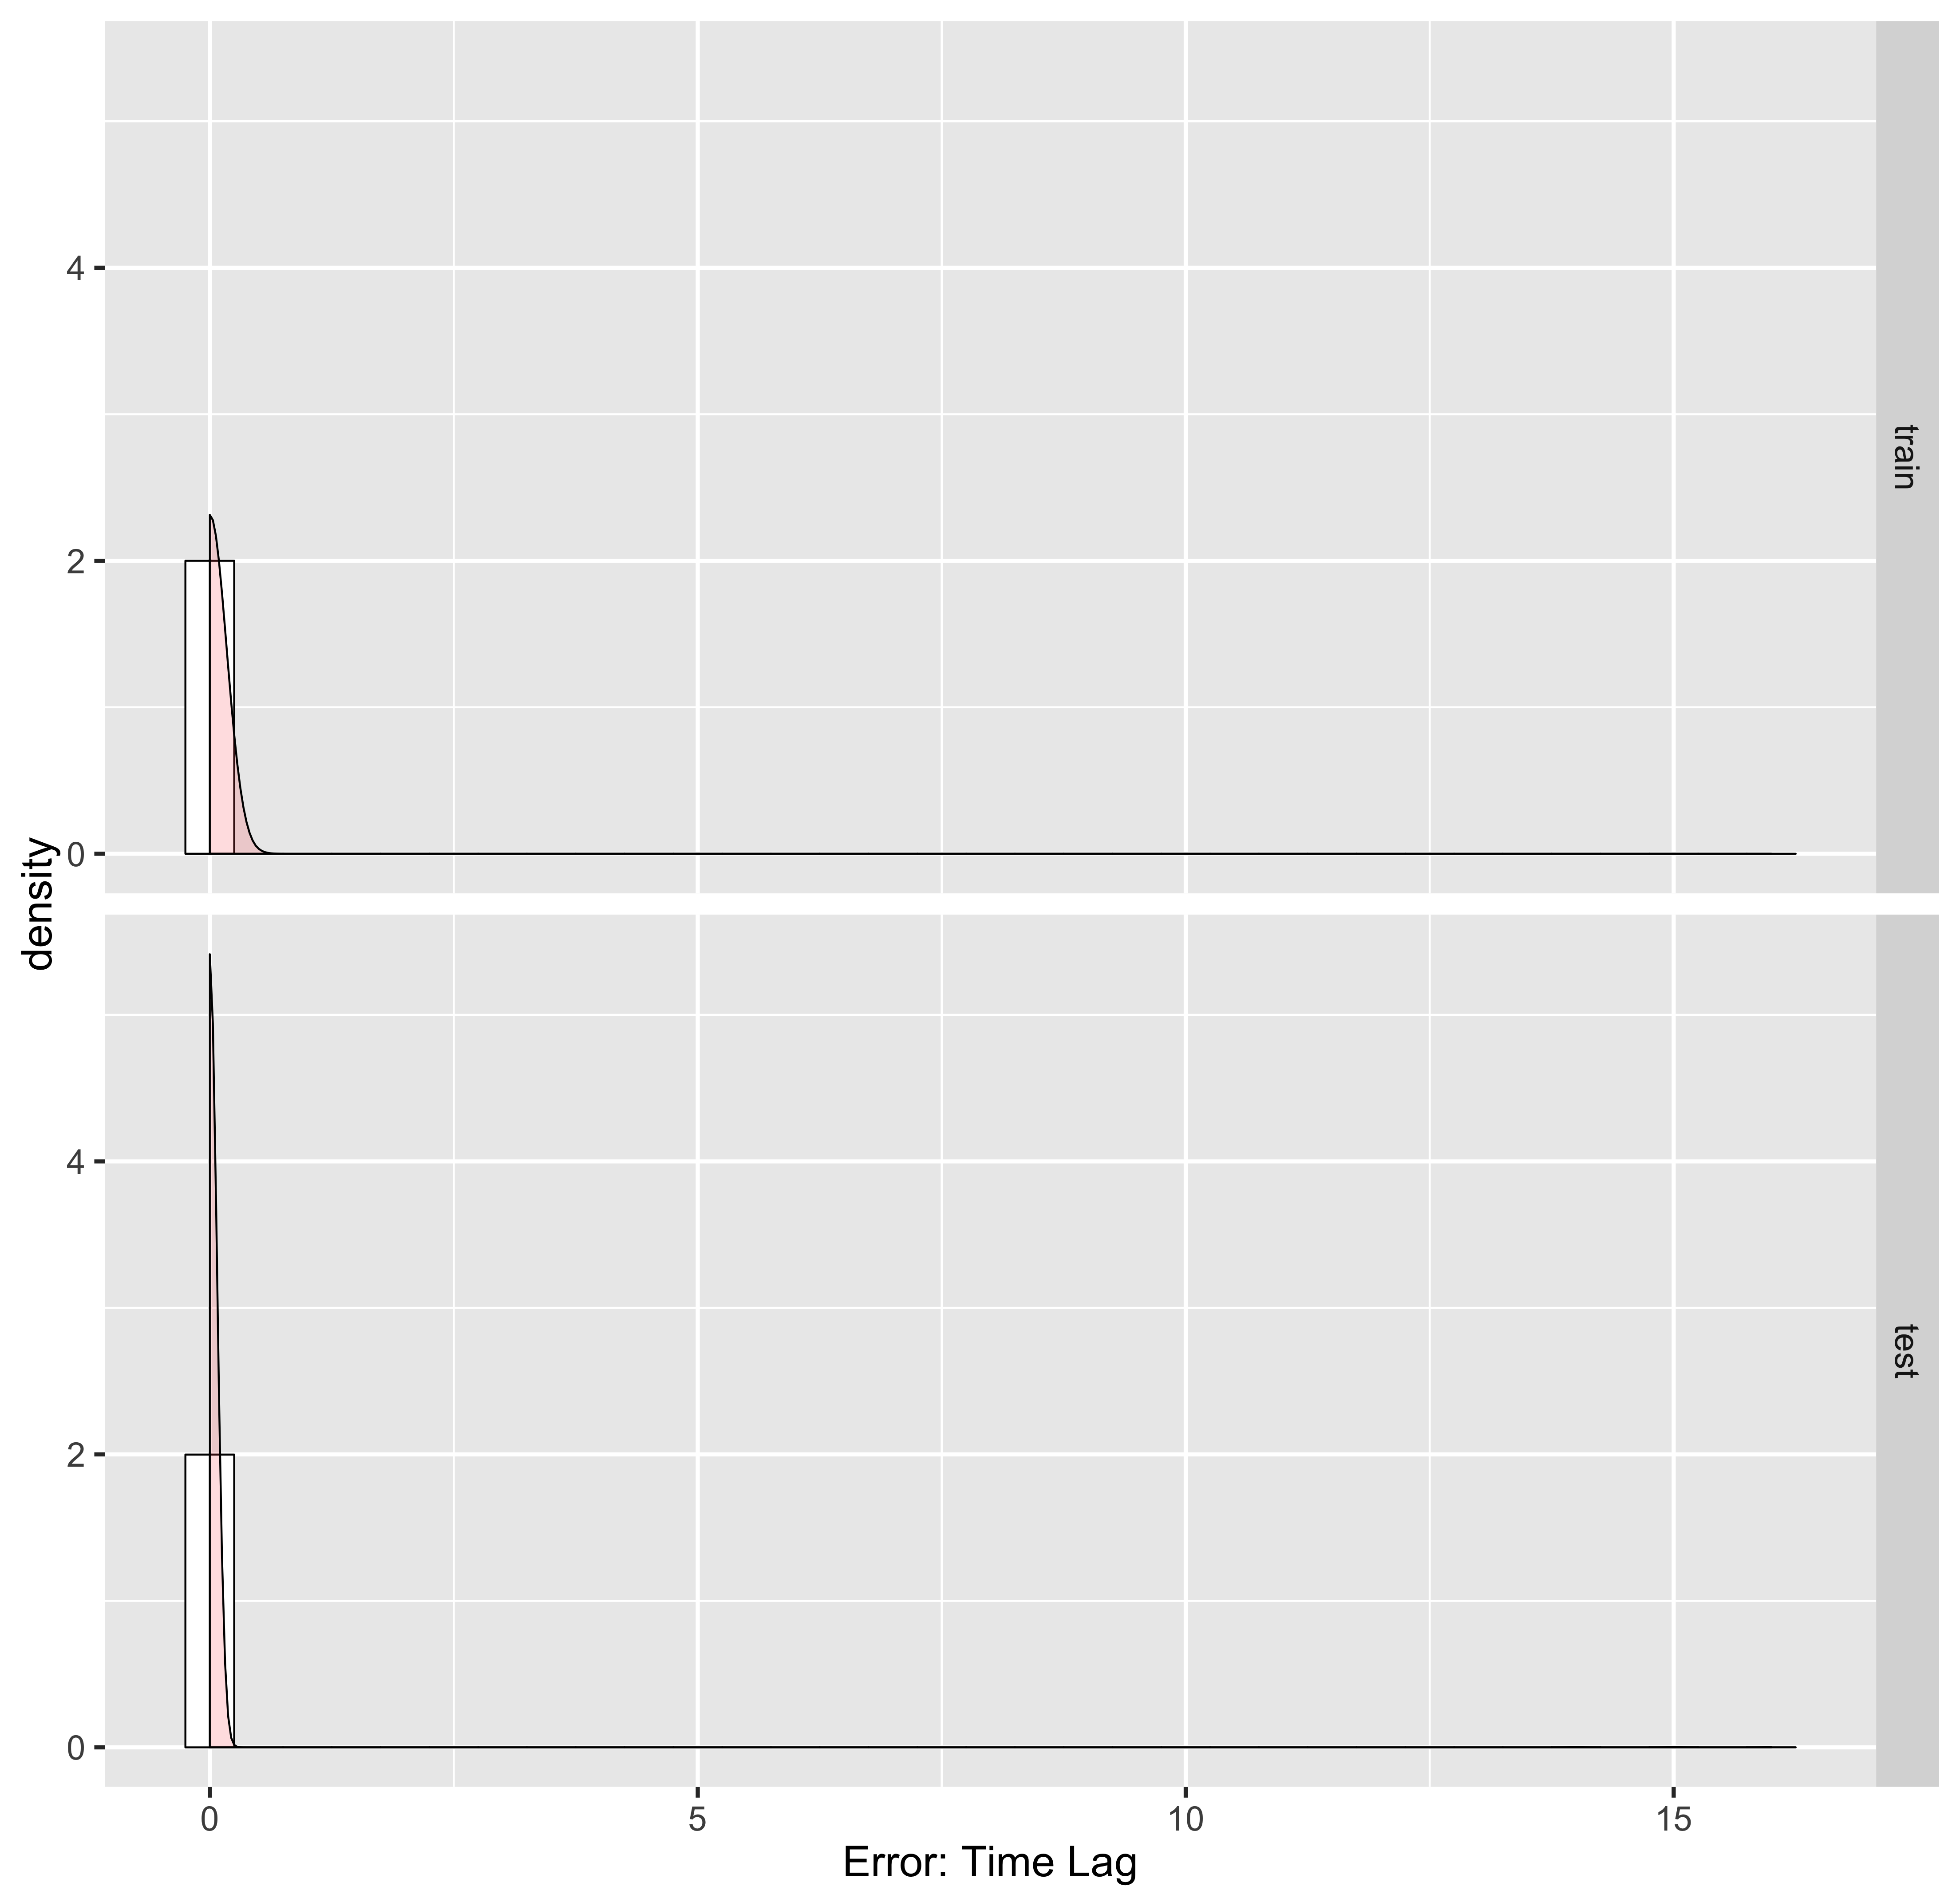
\includegraphics[width=0.5\textwidth]{figures/exp1_hist_errors_timelag.png}}
\vspace{.3in}
\caption{\textbf{Problem I}, Distribution of the time lag prediction error}
\end{figure}



\begin{figure}[h]\label{fig:problem2_scatter}
\vspace{.3in}
\centerline{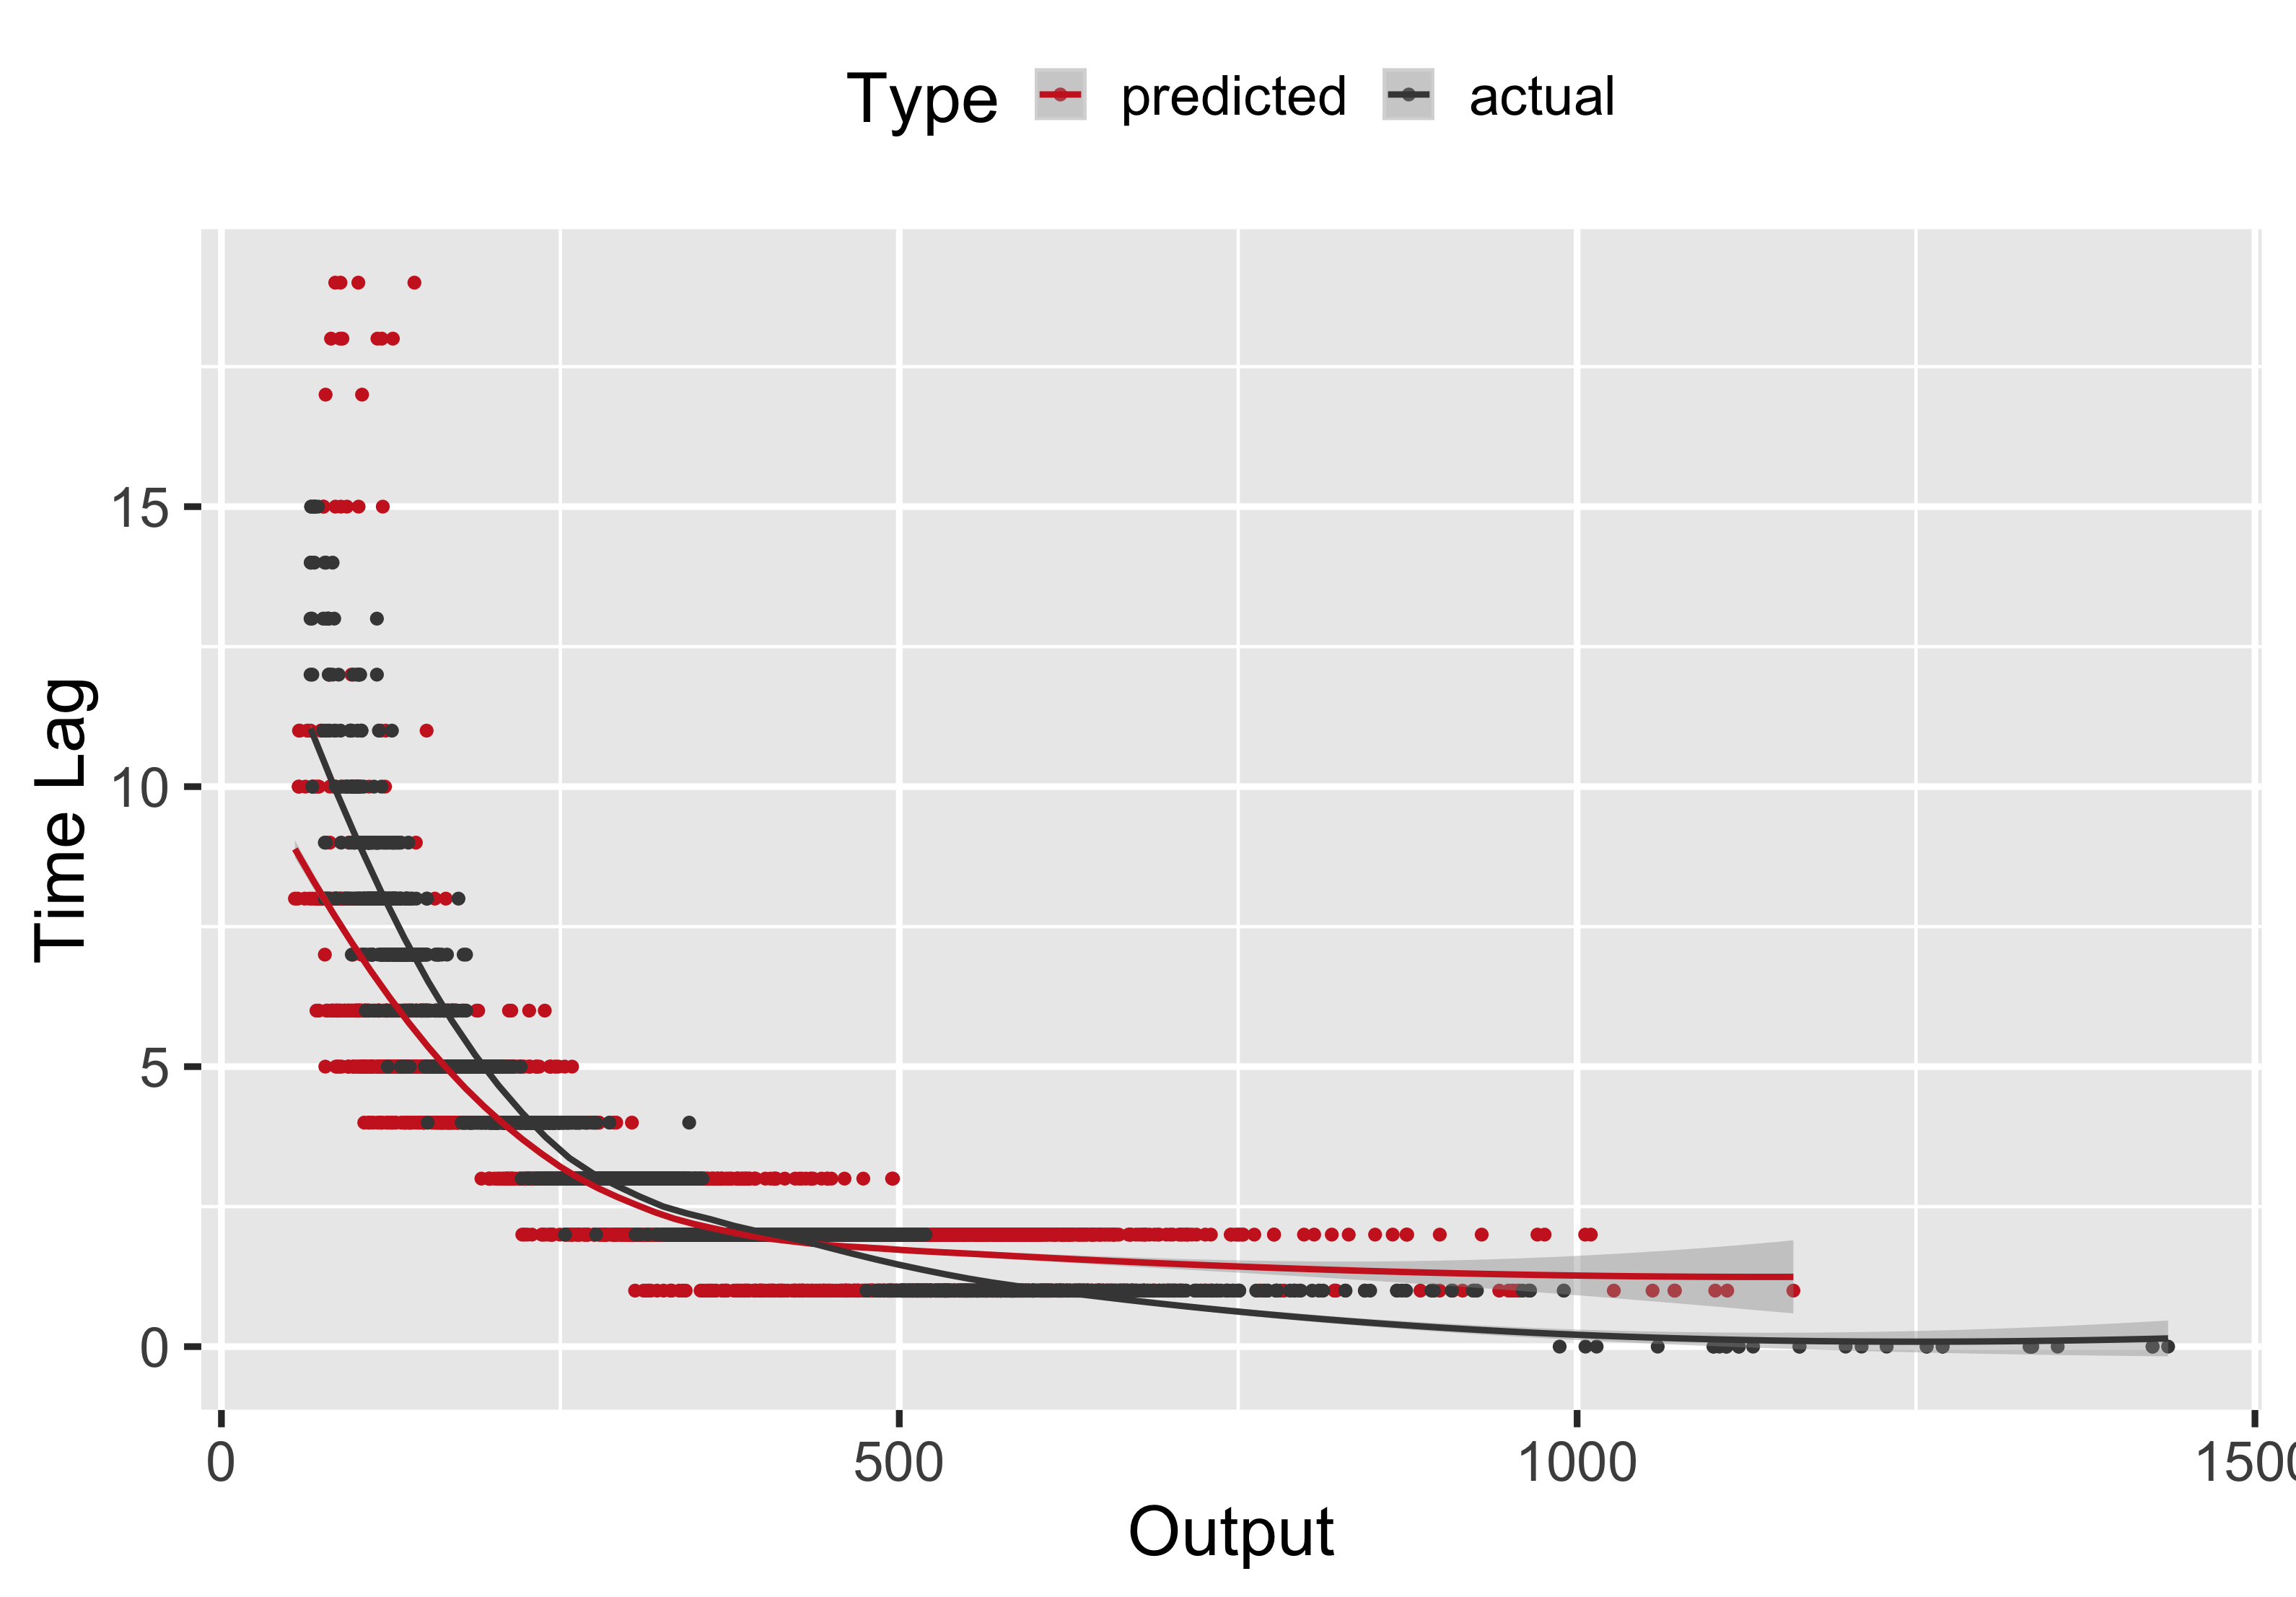
\includegraphics[width=0.5\textwidth]{figures/exp2_scatter_v_tl.png}}
\vspace{.3in}
\caption{\textbf{Problem II}, Output-Time Lag Scatter plot on test data; model predictions in red and actual data in black}
\end{figure}

\begin{figure}[h]\label{fig:problem2_error}
\vspace{.3in}
\centerline{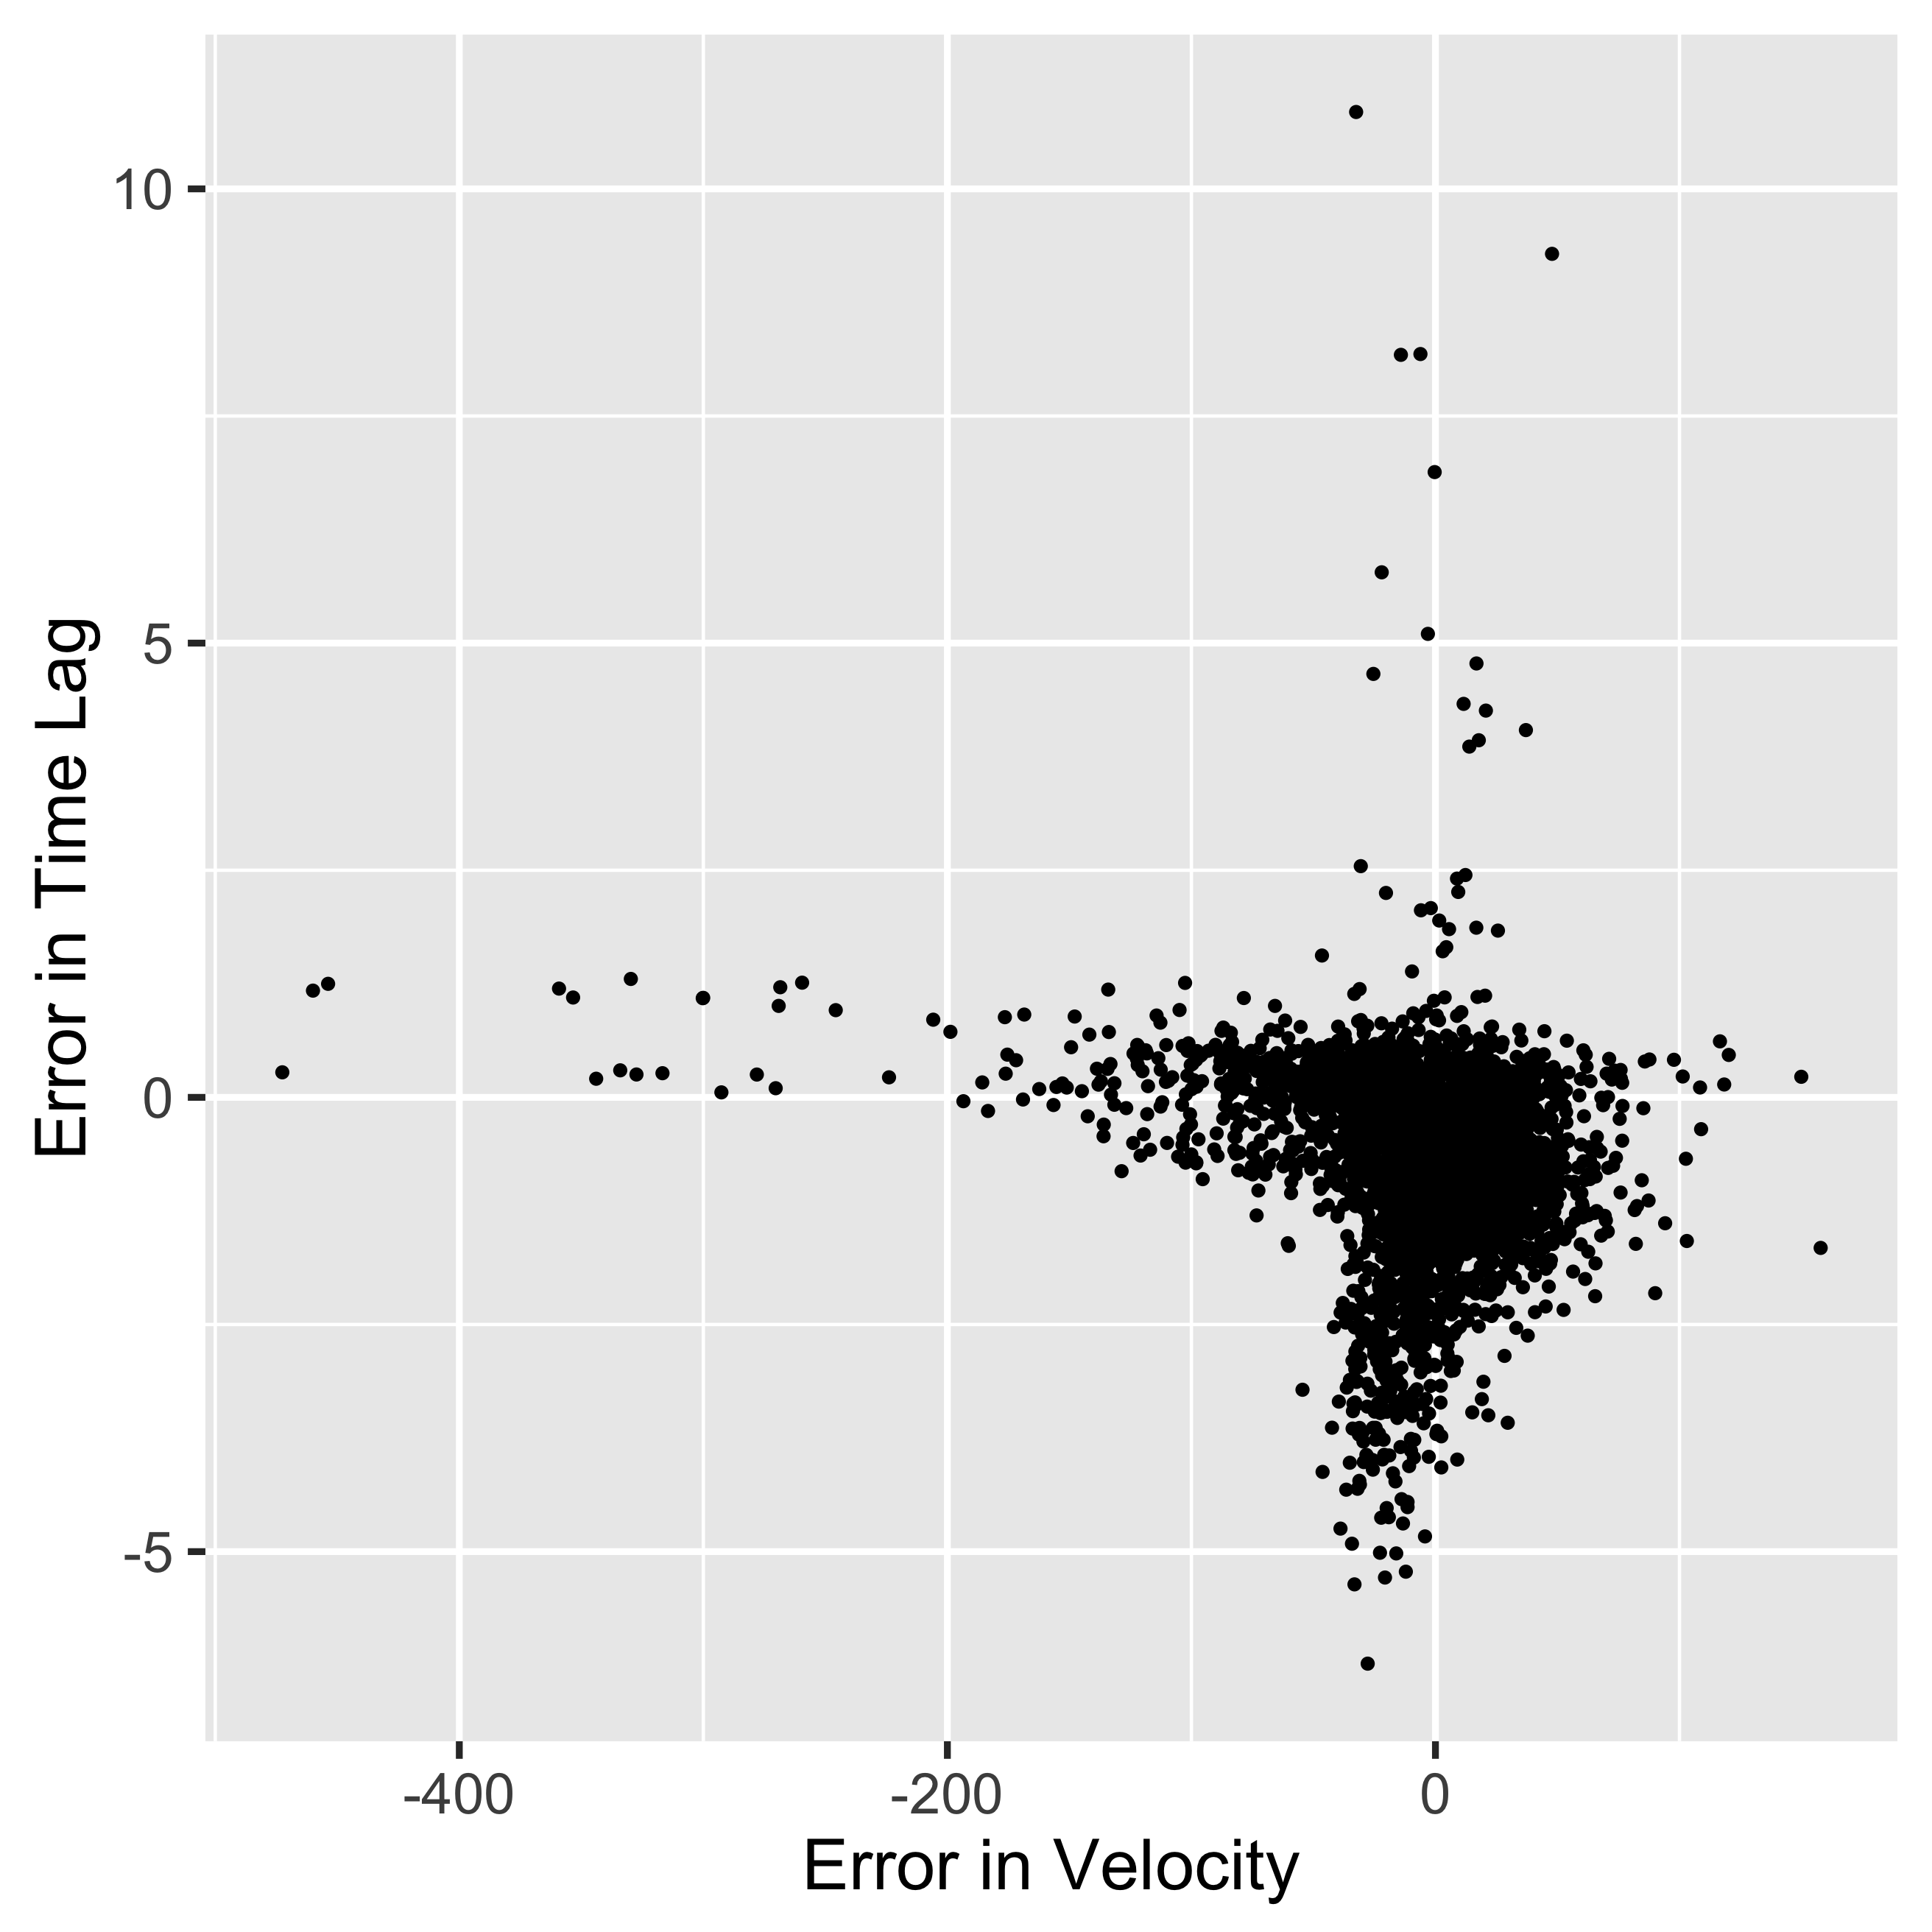
\includegraphics[width=0.5\textwidth]{figures/exp2_scatter_errors_test.png}}
\vspace{.3in}
\caption{\textbf{Problem II}, Error Scatter plot on test data}
\end{figure}

\begin{figure}[h]\label{fig:problem2_curves}
\vspace{.3in}
\centerline{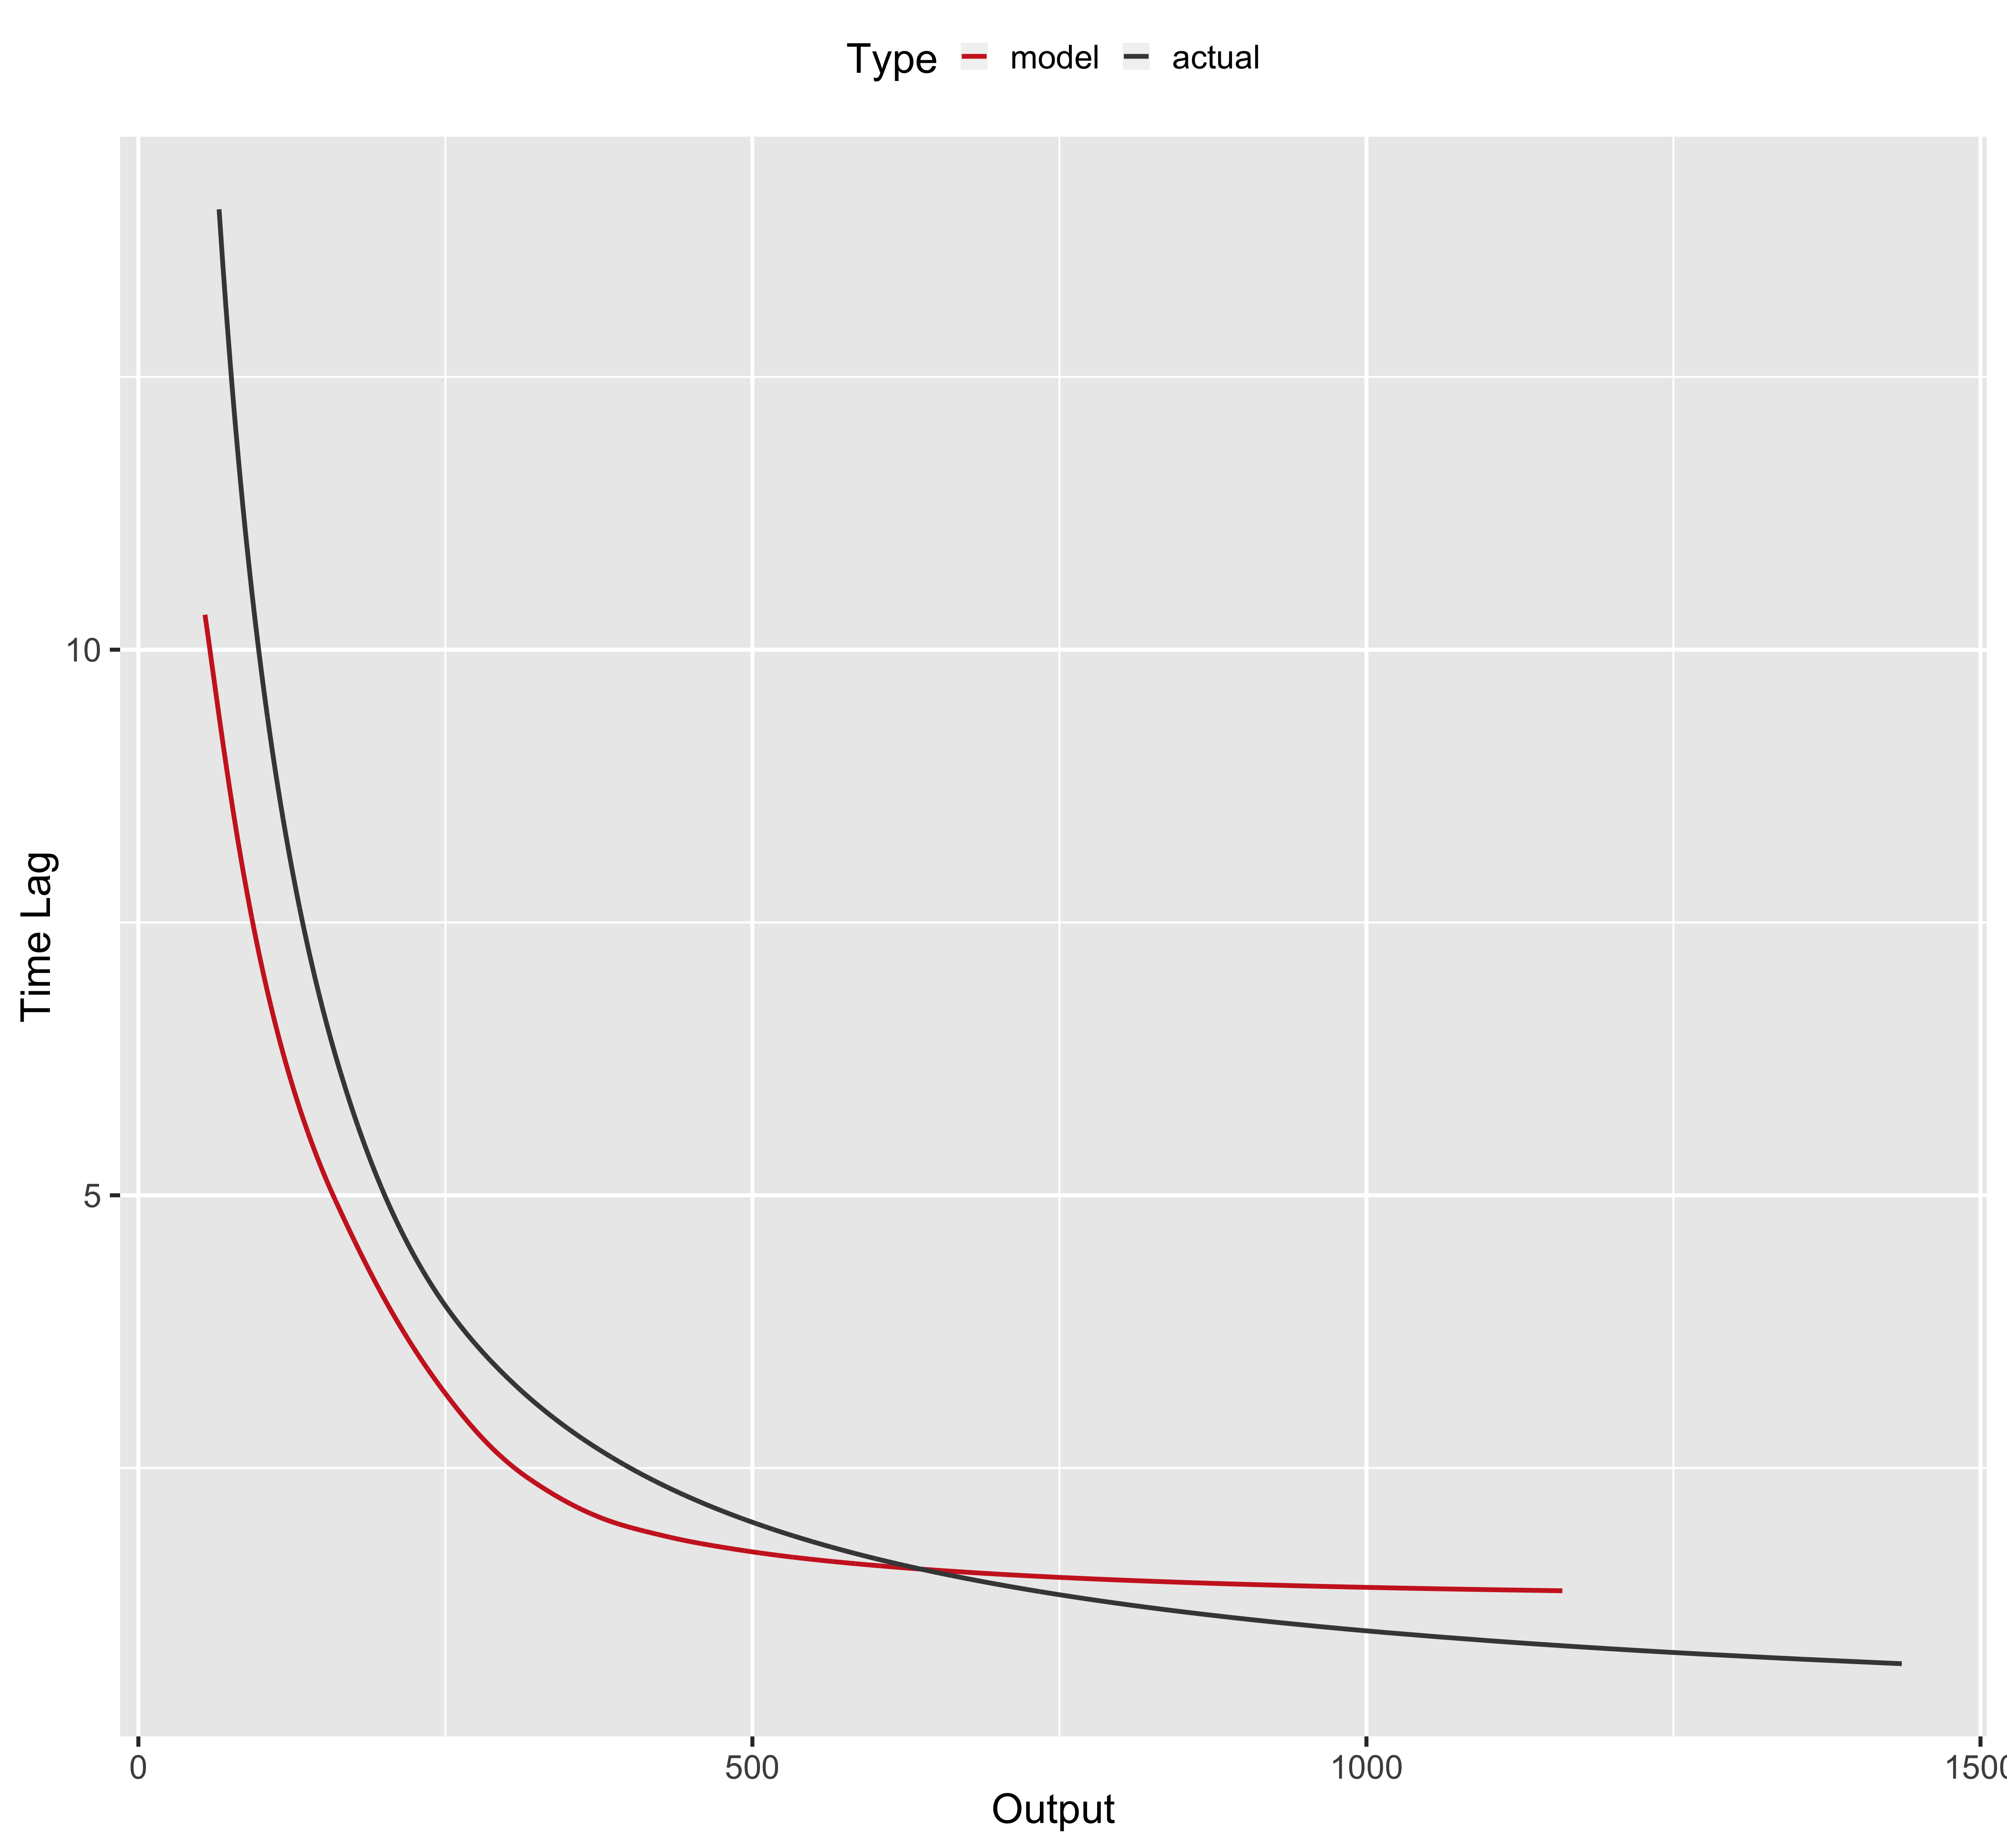
\includegraphics[width=0.5\textwidth]{figures/exp2_predictive_curves.png}}
\vspace{.3in}
\caption{\textbf{Problem II}, Output vs Time Lag Relationship}
\end{figure}



\begin{figure}[h]
\vspace{.3in}
\centerline{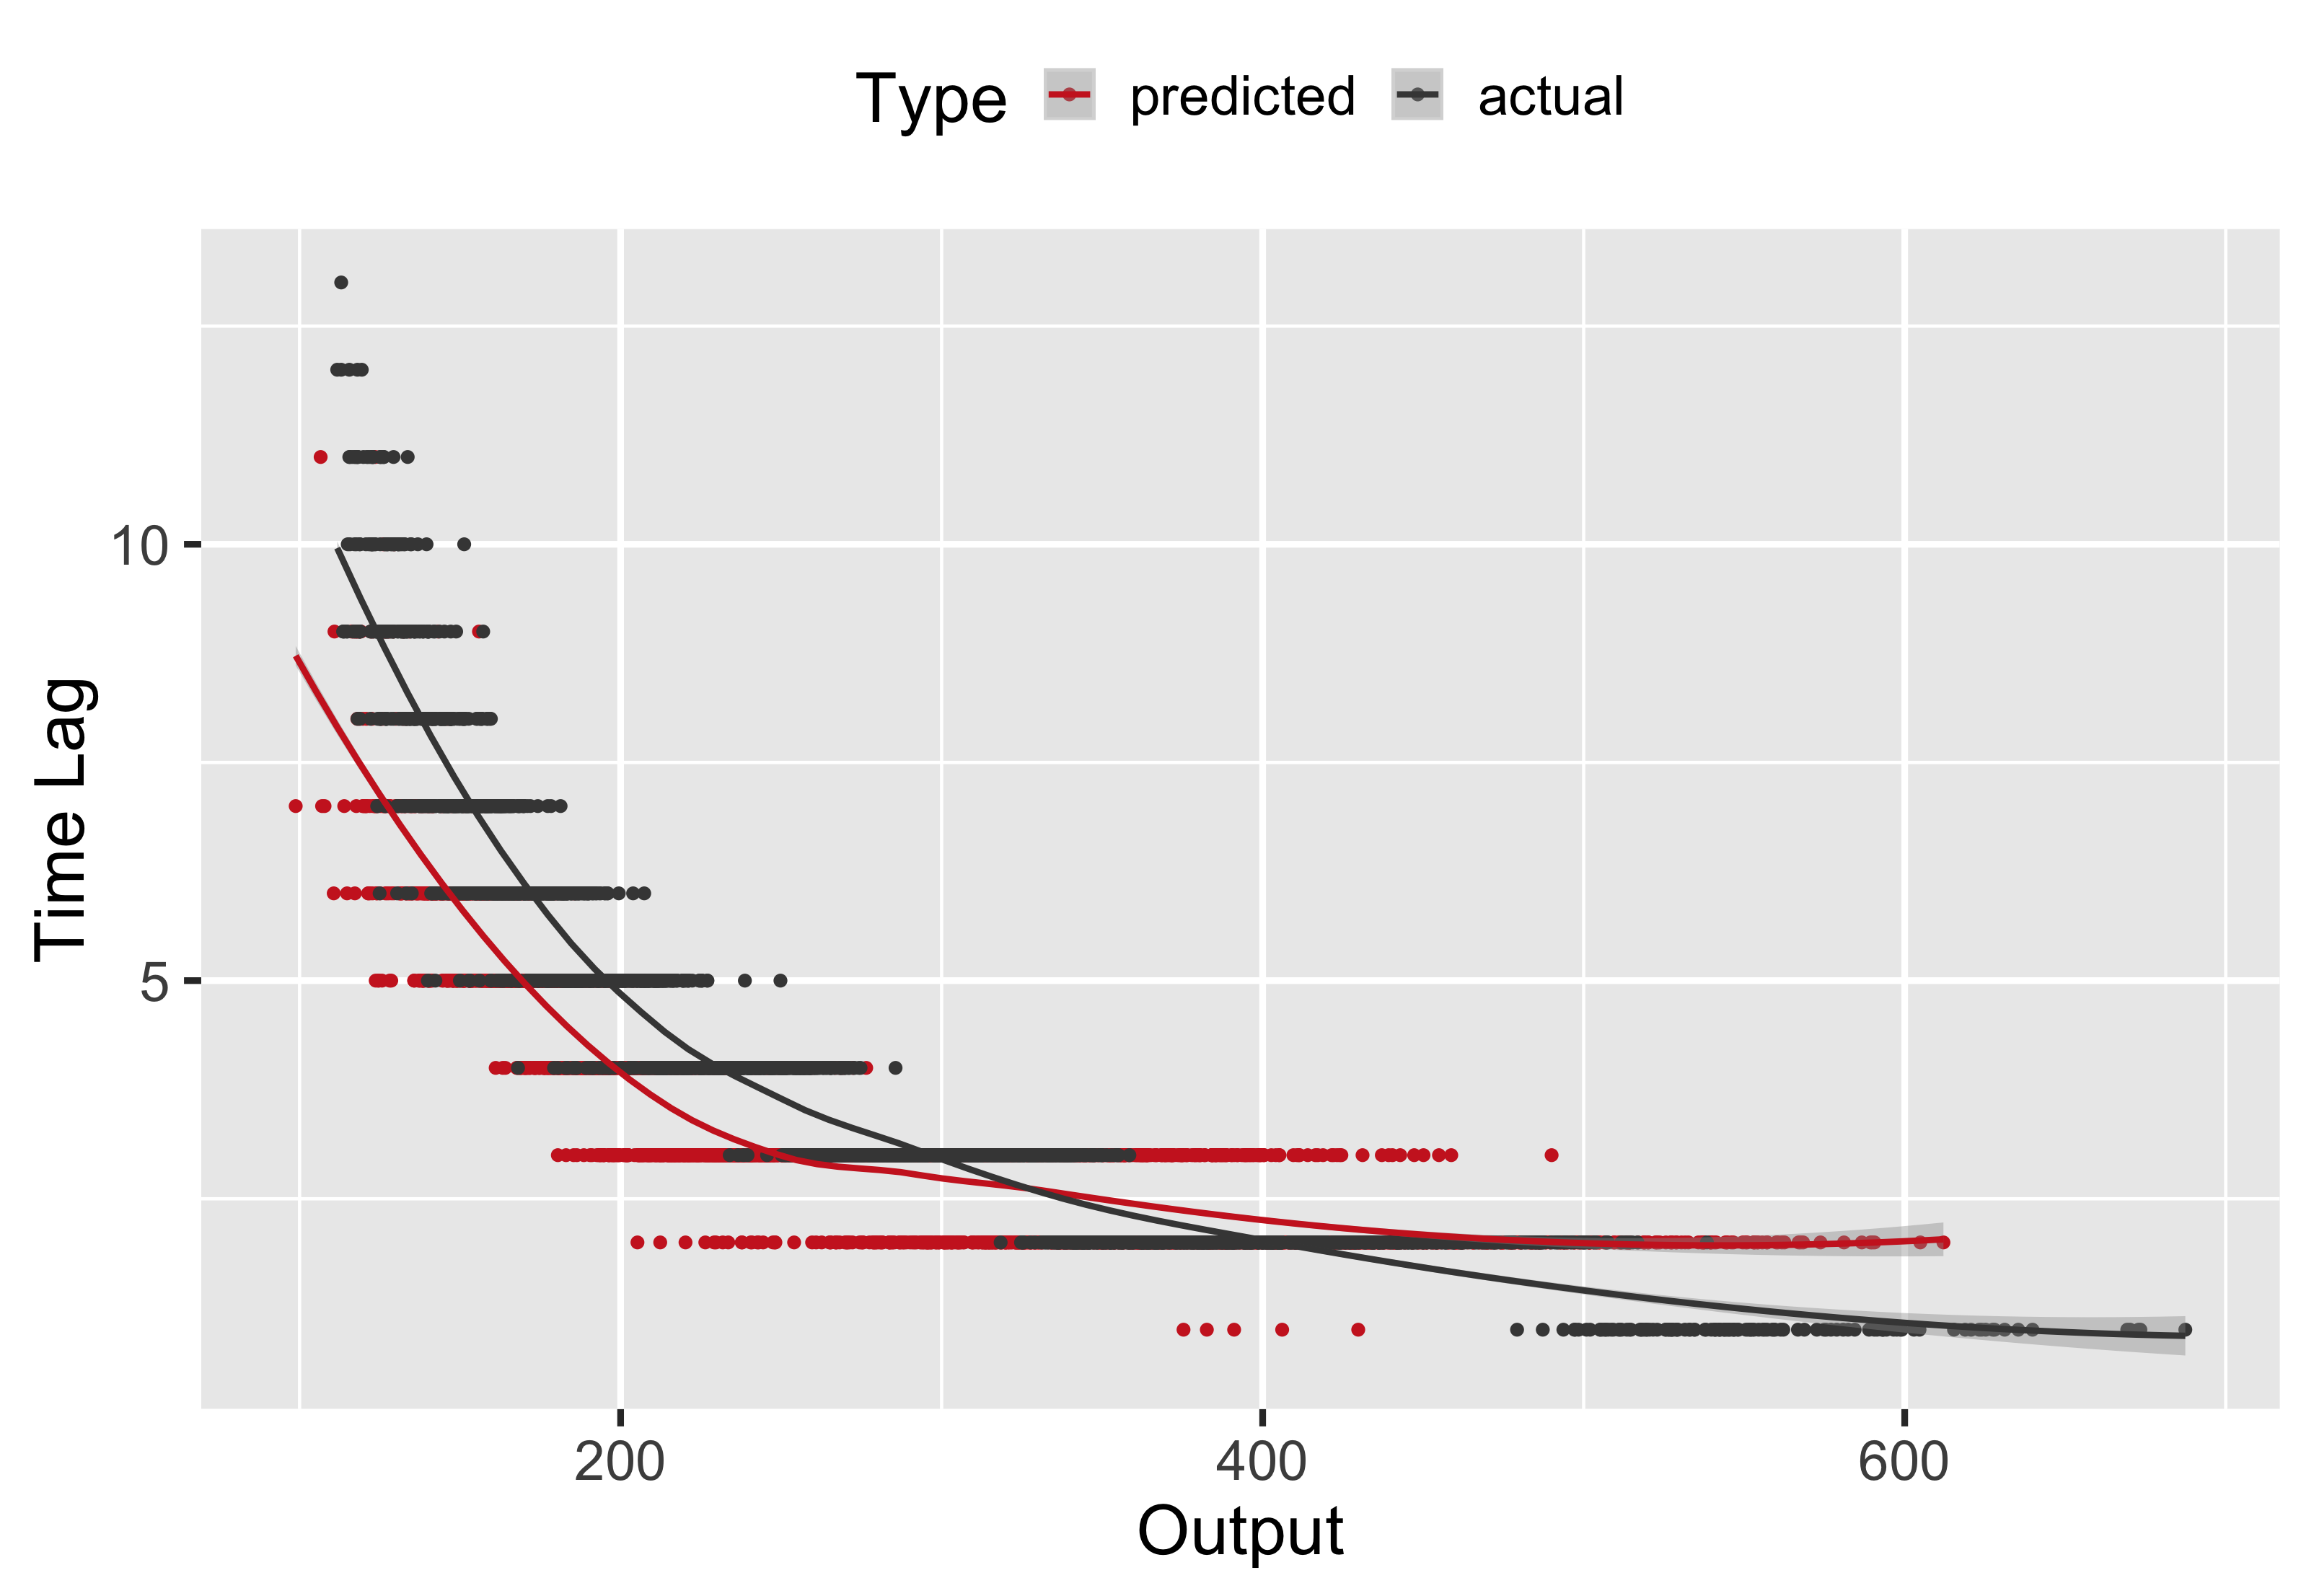
\includegraphics[width=0.5\textwidth]{figures/exp3_scatter_v_tl.png}}
\vspace{.3in}
\caption{\textbf{Problem III}, Output-Time Lag Scatter plot; model predictions in red and actual data in black}
\end{figure}

\begin{figure}[h]
\vspace{.3in}
\centerline{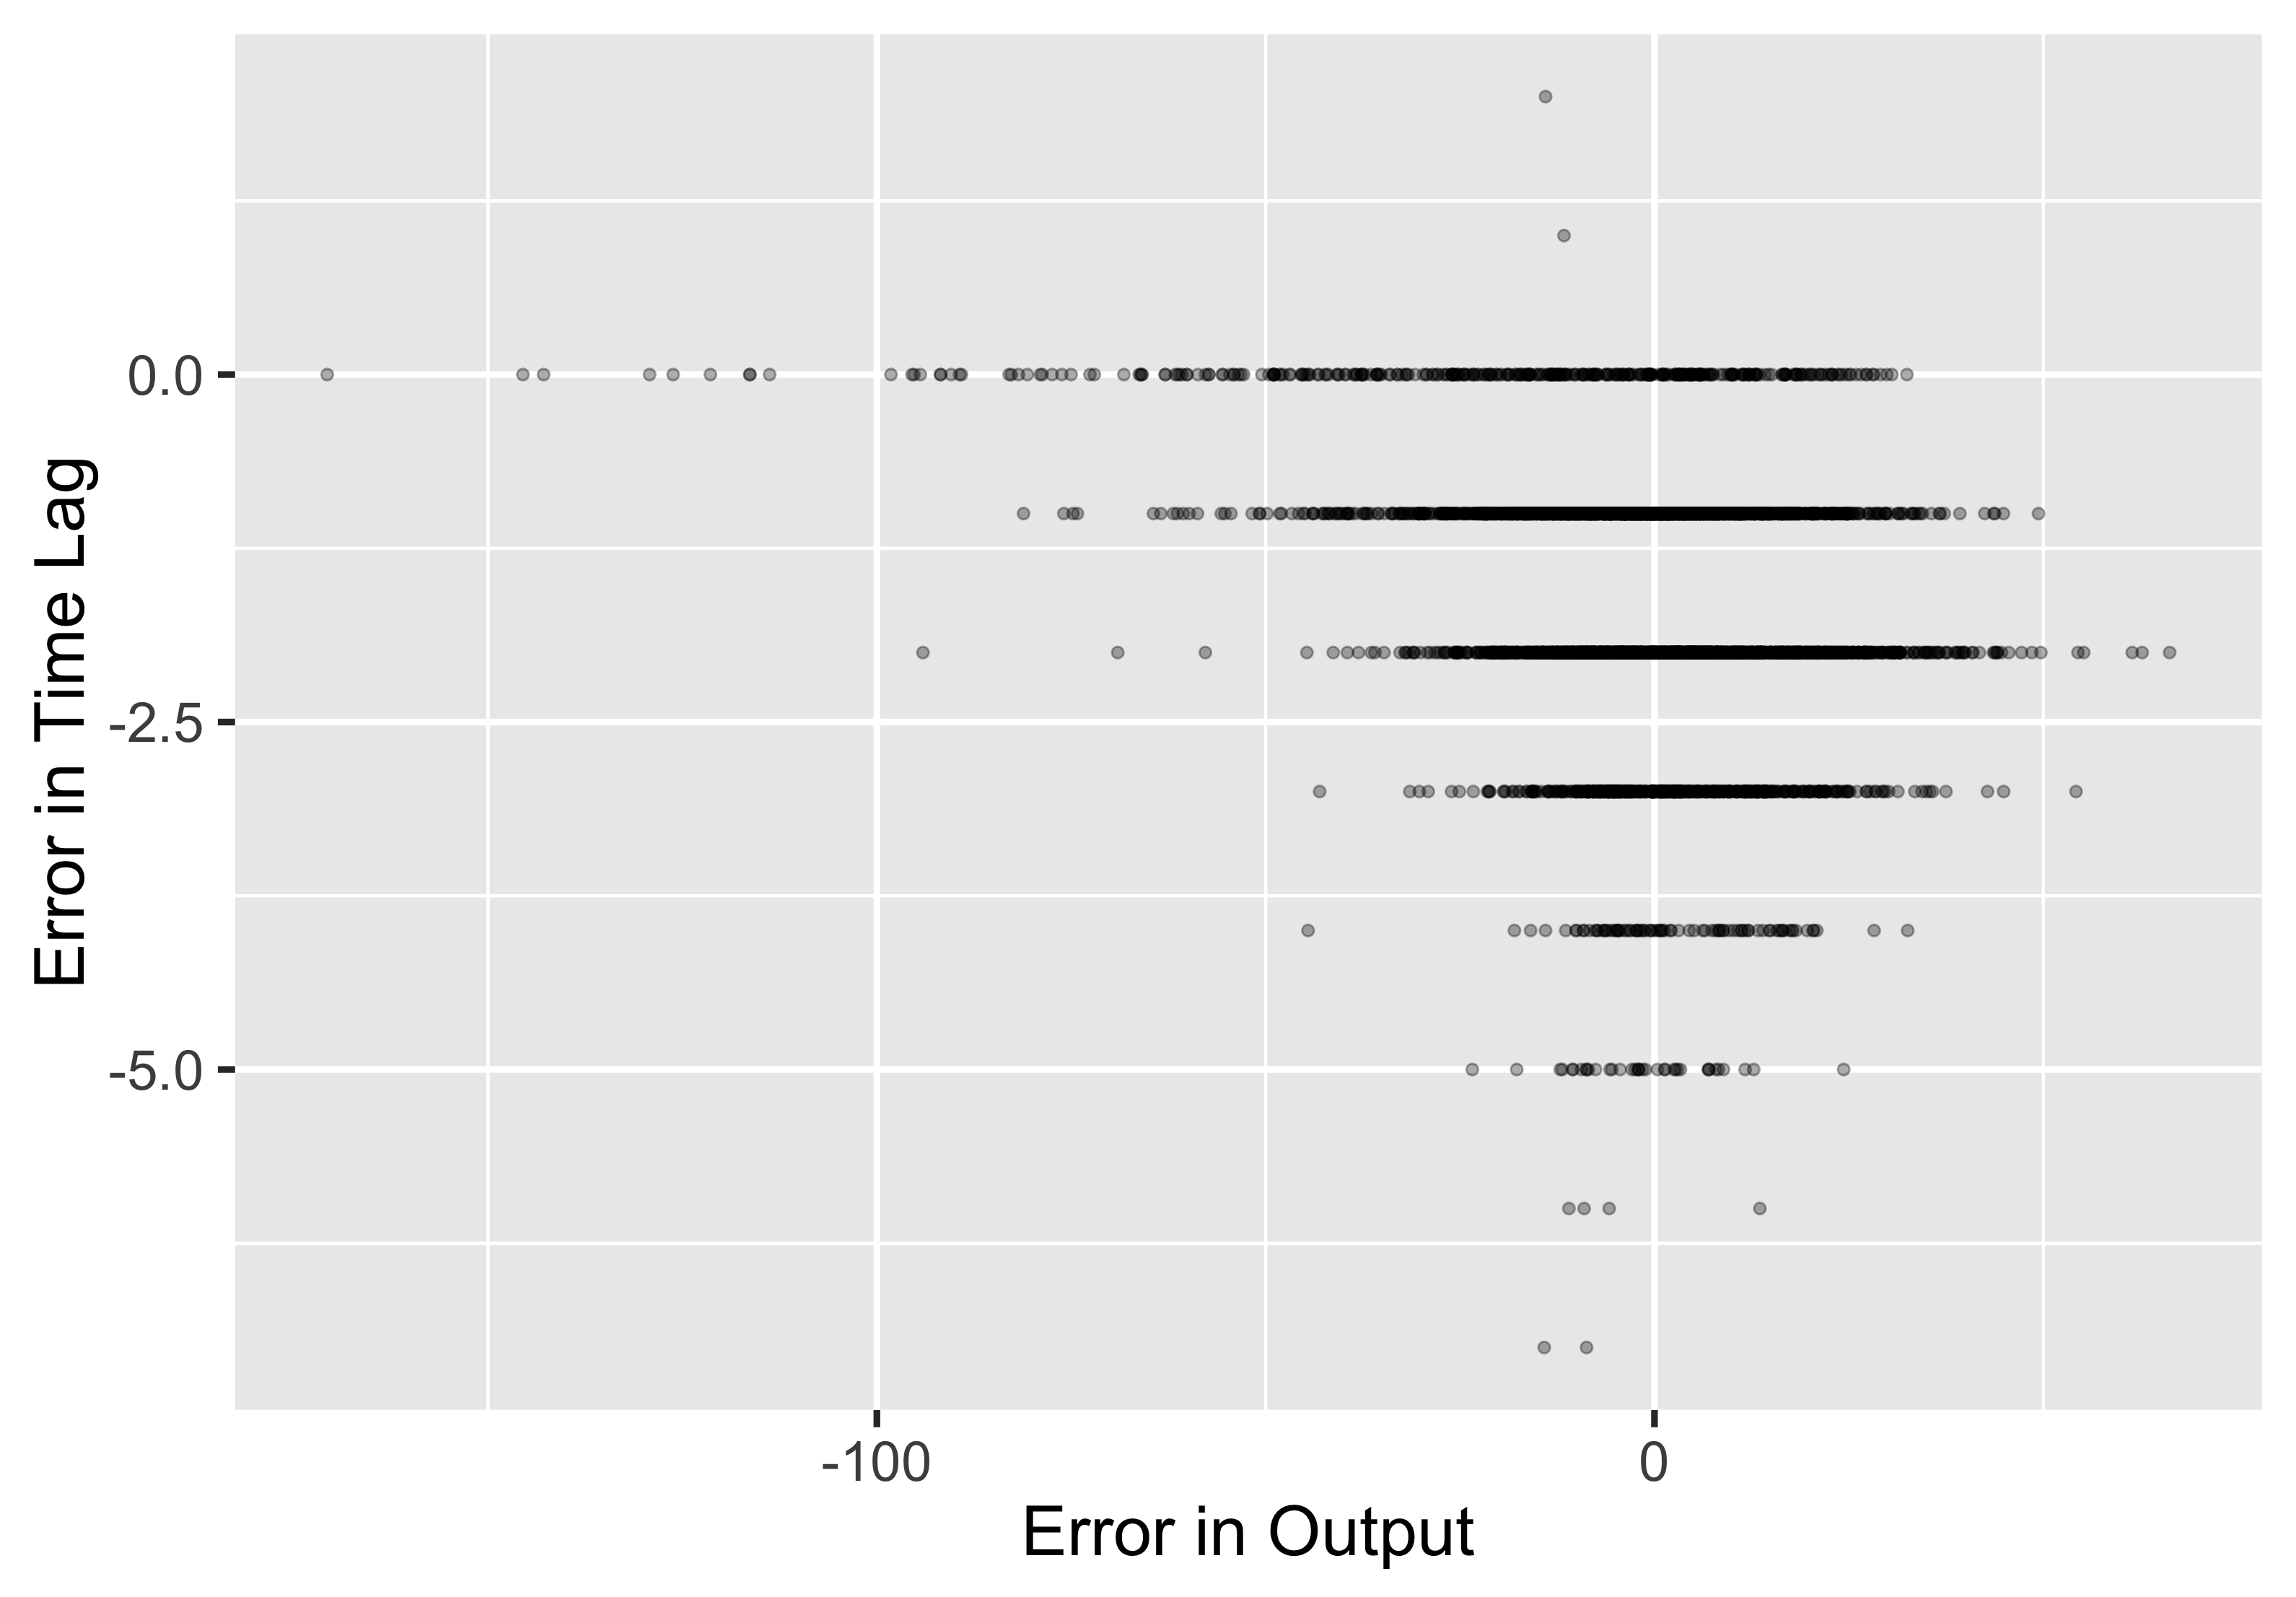
\includegraphics[width=0.5\textwidth]{figures/exp3_scatter_errors_test.png}}
\vspace{.3in}
\caption{\textbf{Problem III}, Error Scatter plot on test data}
\end{figure}

\begin{figure}[h]
\vspace{.3in}
\centerline{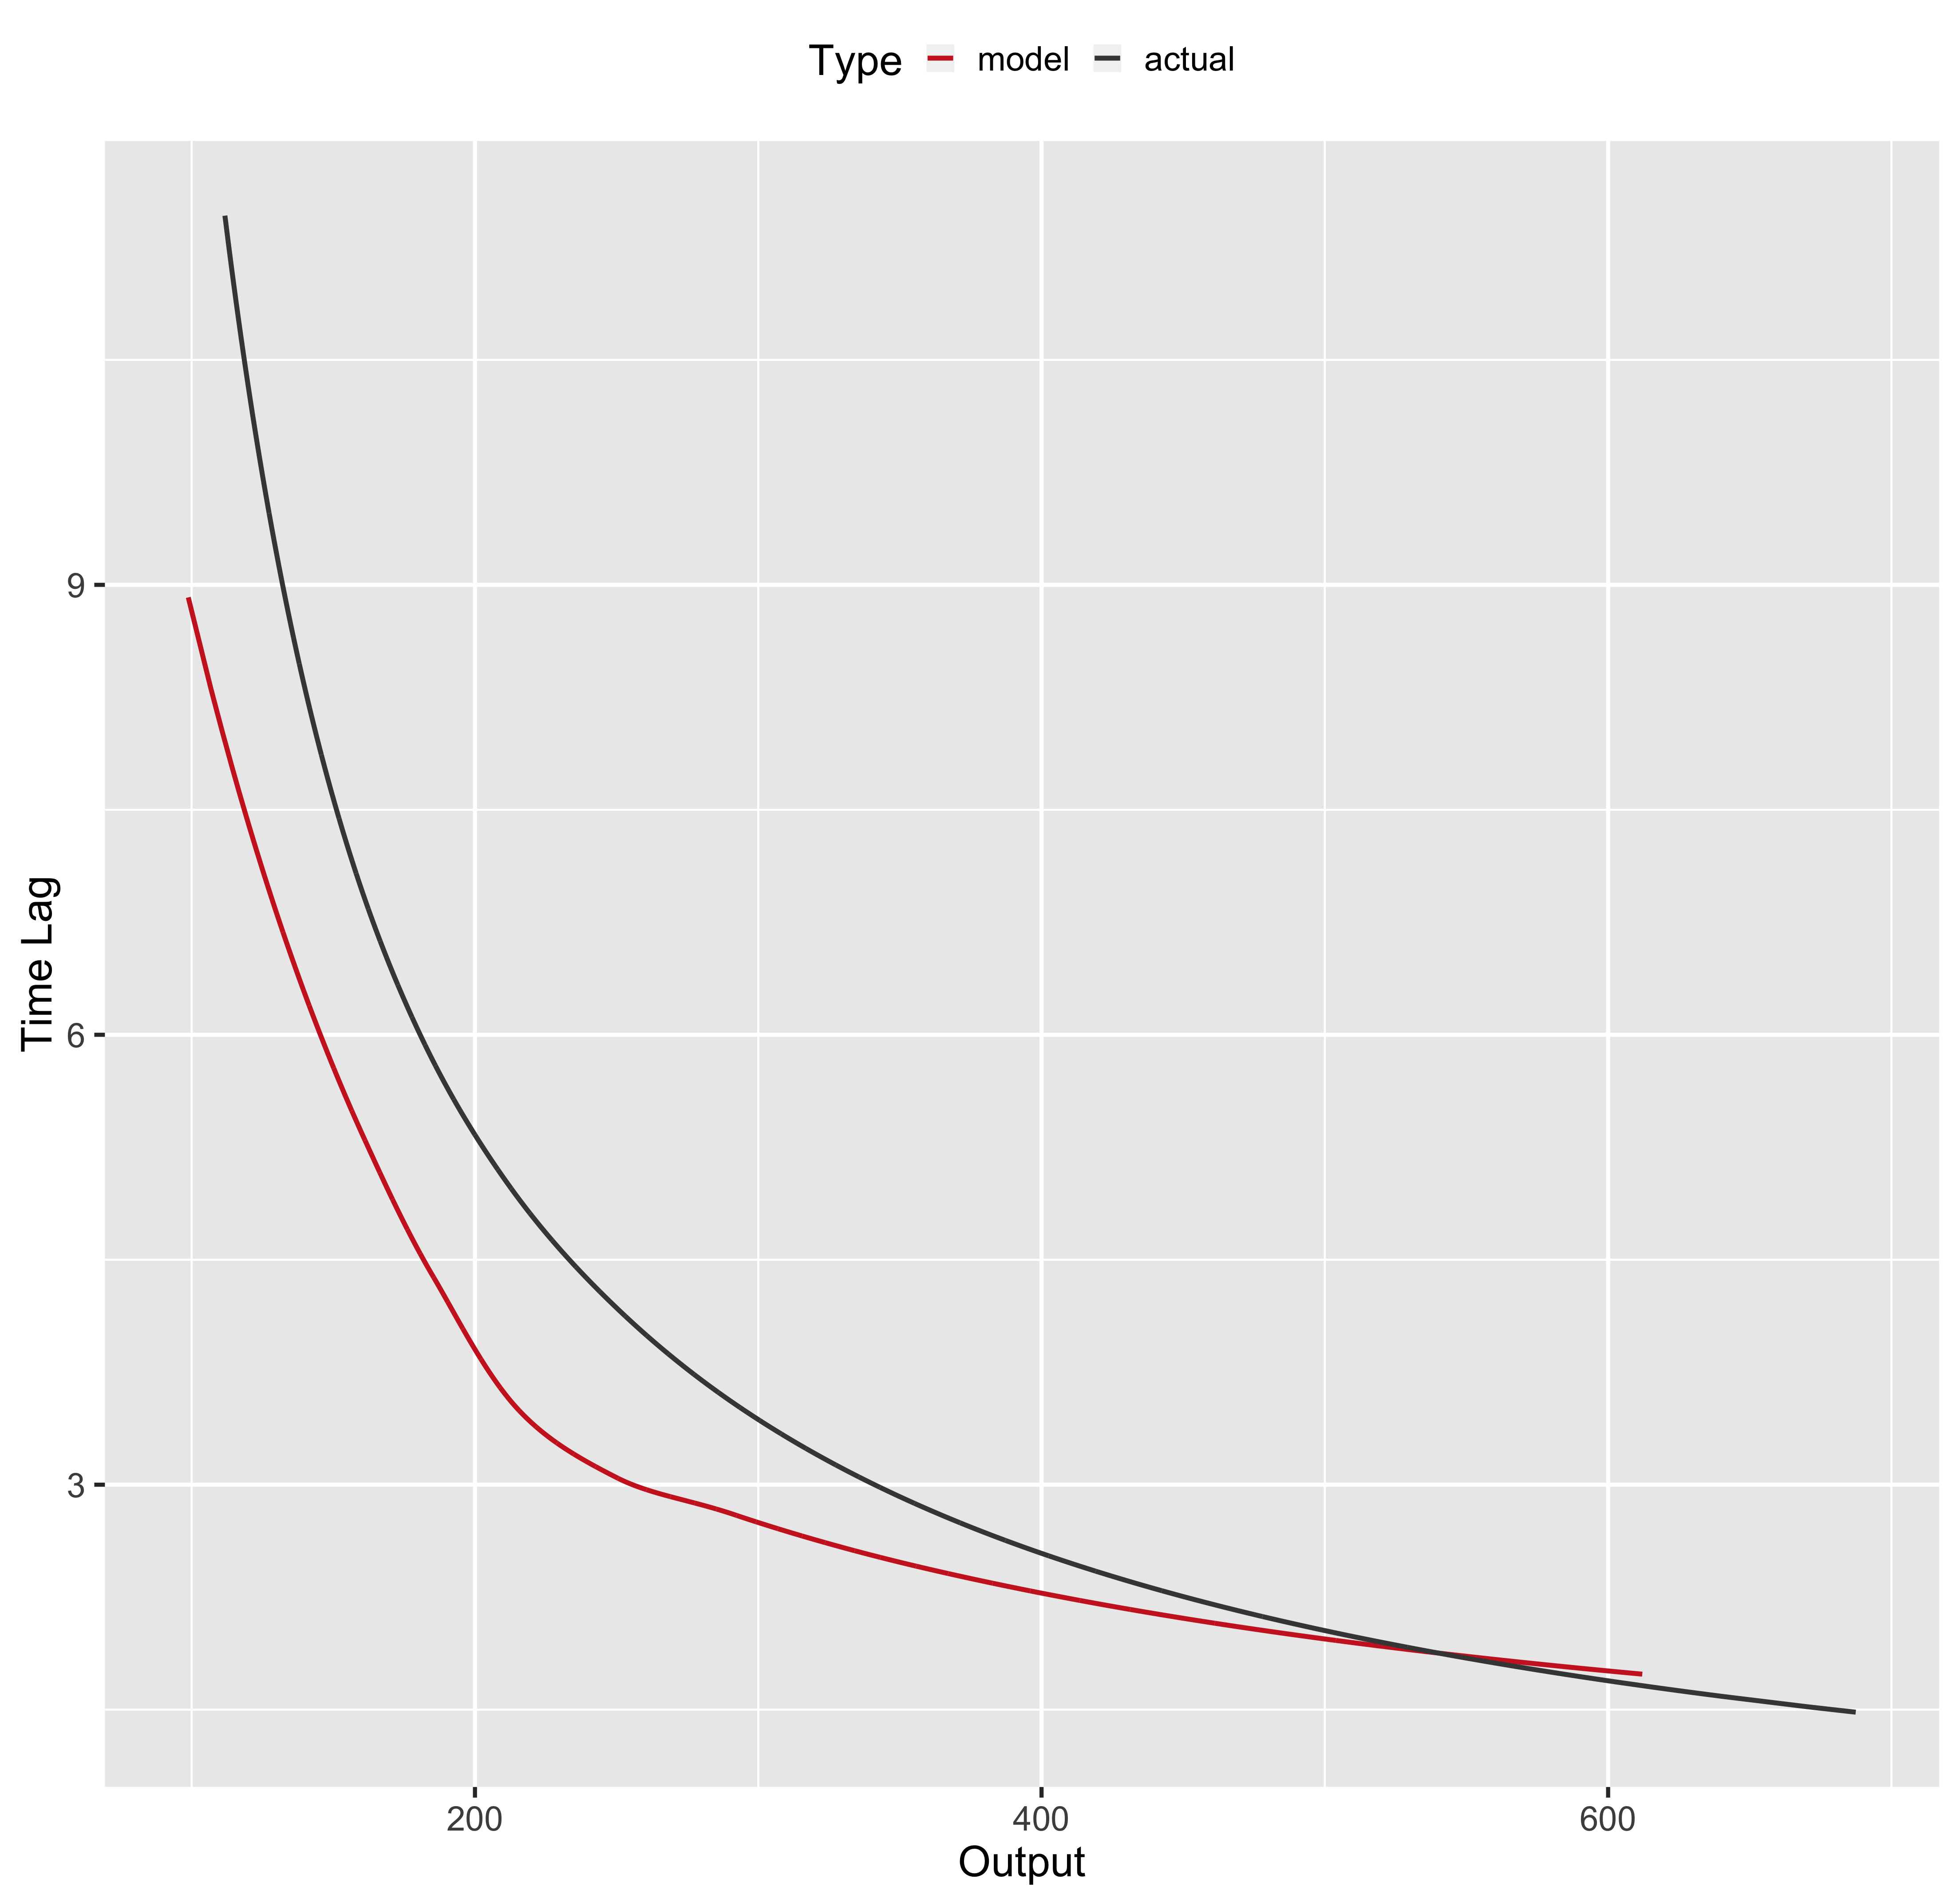
\includegraphics[width=0.5\textwidth]{figures/exp3_predictive_curves.png}}
\vspace{.3in}
\caption{\textbf{Problem III}, Output vs Time Lag Relationship}
\end{figure}


\begin{figure}[h]
\vspace{.3in}
\centerline{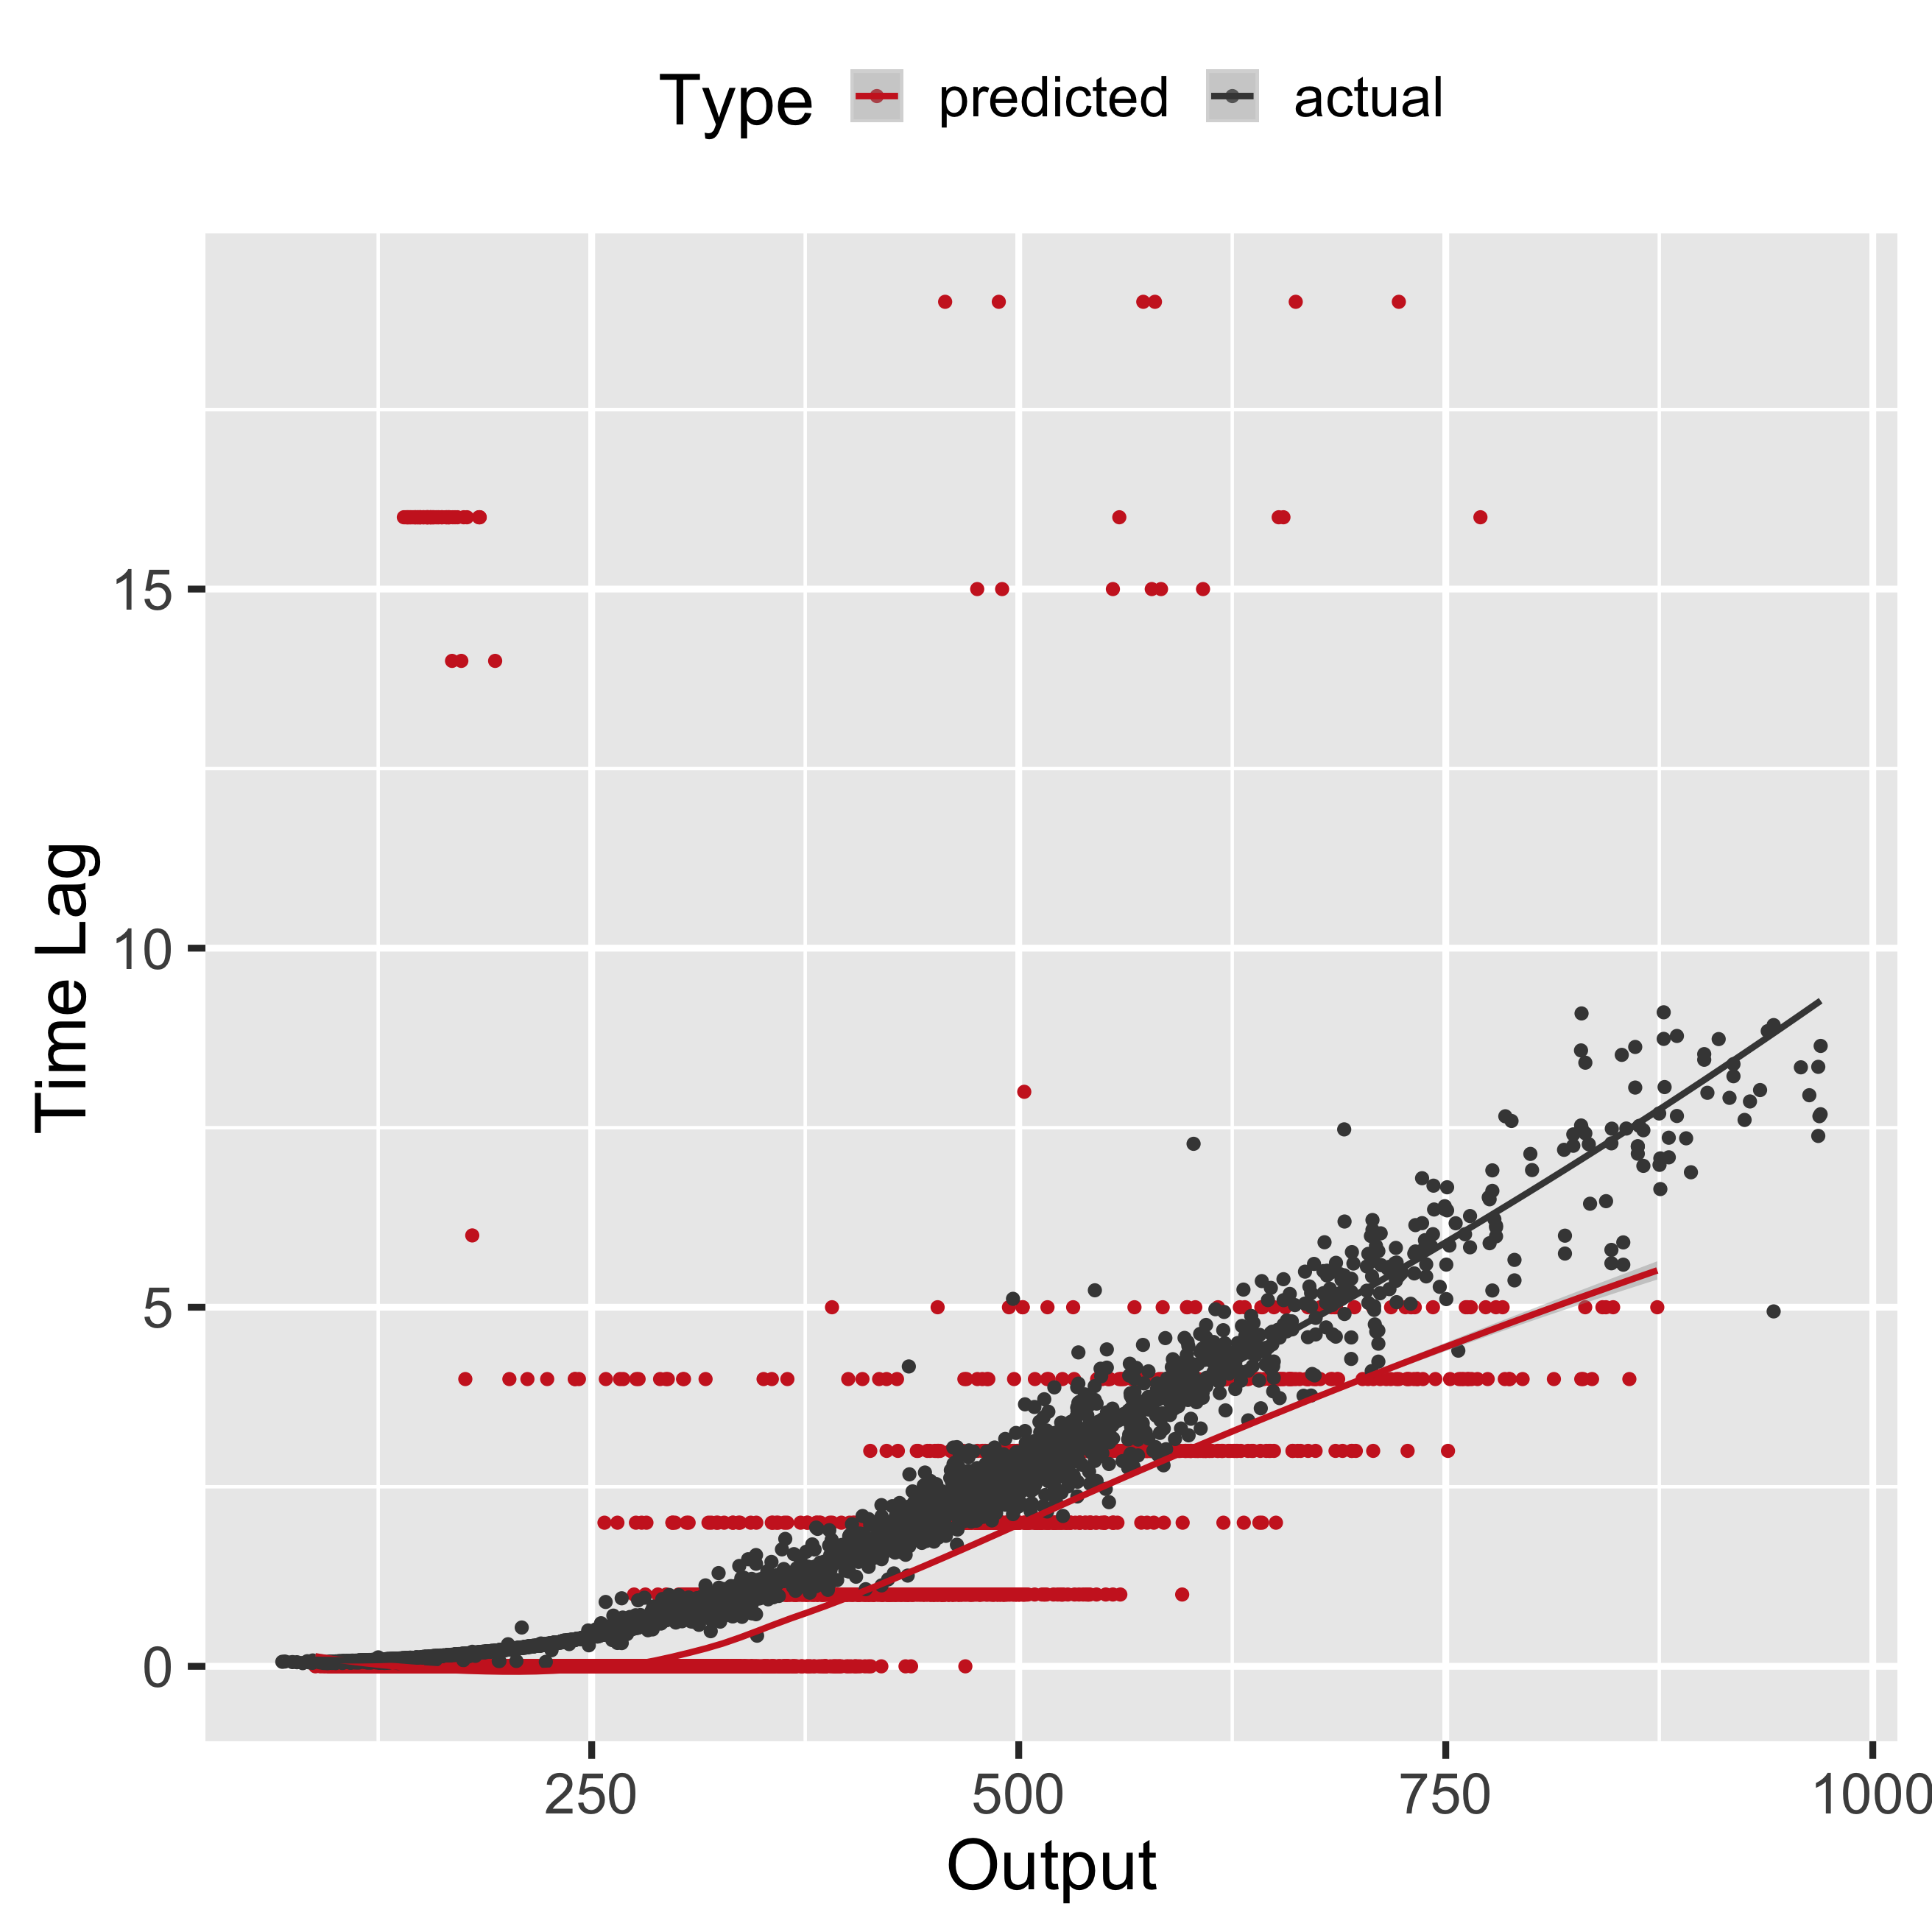
\includegraphics[width=0.5\textwidth]{figures/exp4_scatter_v_tl.png}}
\vspace{.3in}
\caption{\textbf{Problem IV}, Output-Time Lag Scatter plot; model predictions in red and actual data in black}
\end{figure}

\begin{figure}[h]
\vspace{.3in}
\centerline{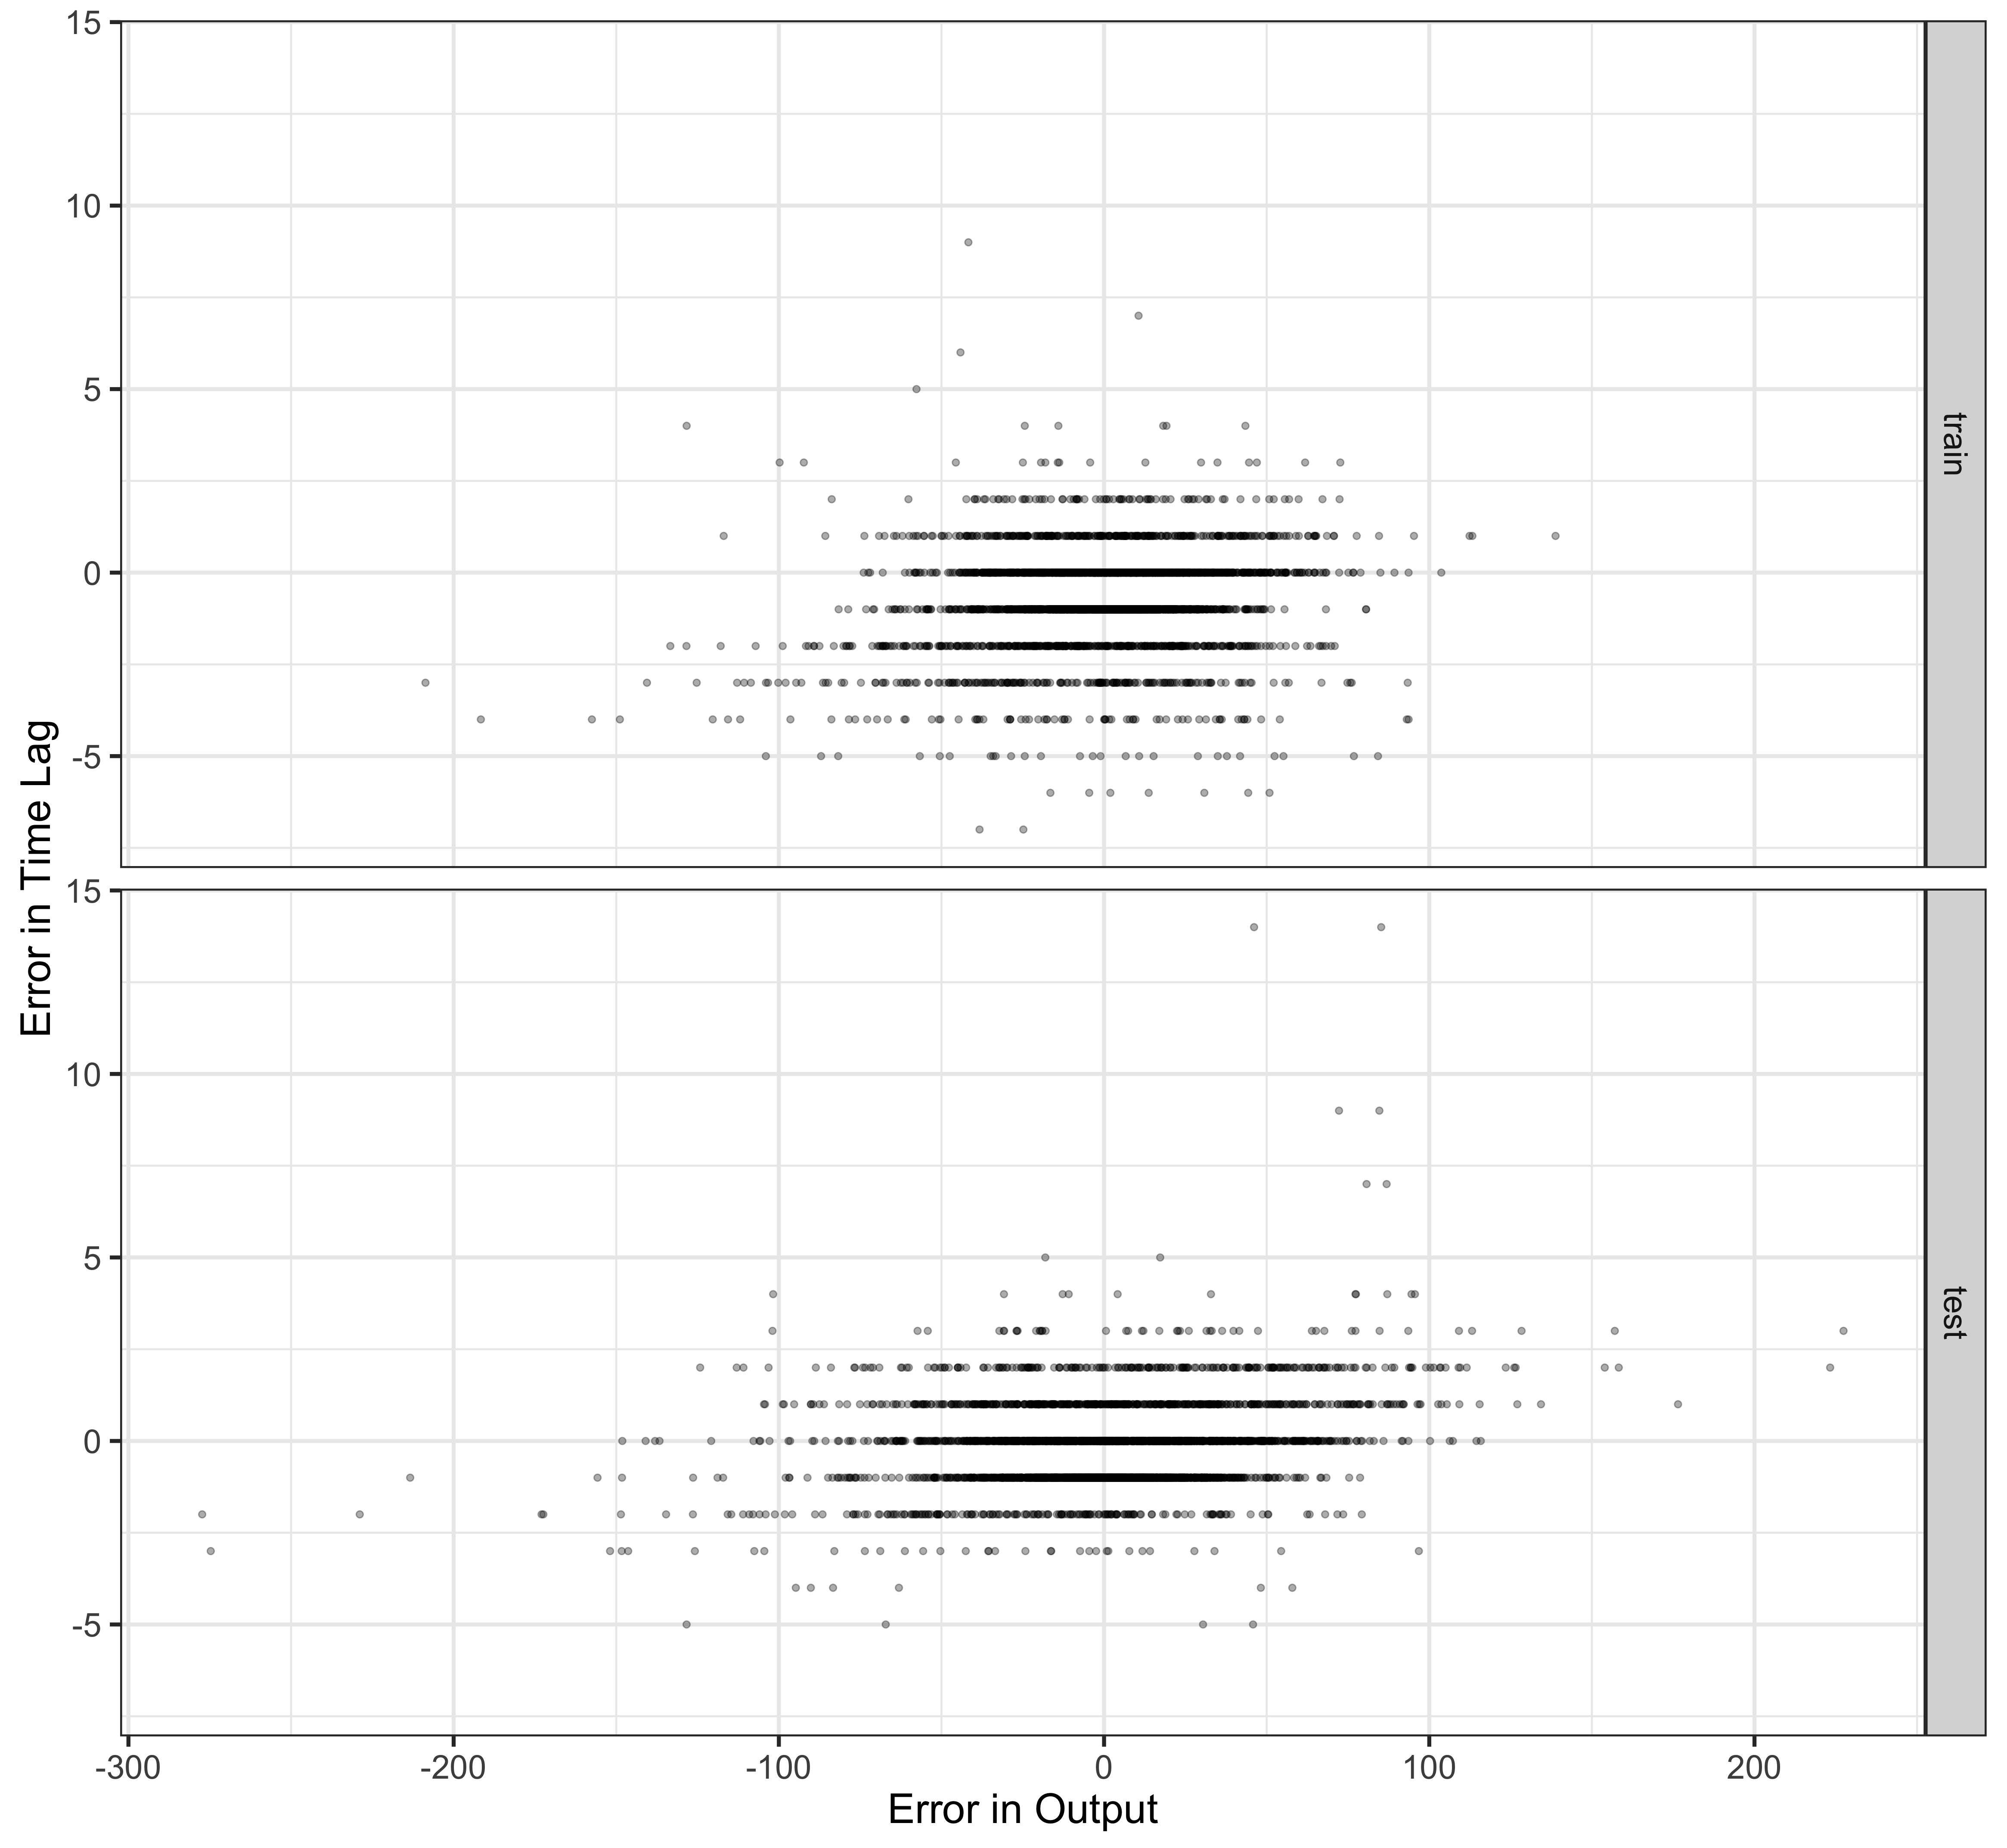
\includegraphics[width=0.5\textwidth]{figures/exp4_scatter_errors_test.png}}
\vspace{.3in}
\caption{\textbf{Problem IV}, Error Scatter plot on test data}
\end{figure}

\subsubsection*{Acknowledgements}

Use the unnumbered third level heading for the acknowledgements.  All
acknowledgements go at the end of the paper.

\subsubsection*{References}

\bibliography{references}

\end{document}
